\documentclass[aps,prx,twocolumn,amsmath,amssymb,superscriptaddress,floatfix,longbibliography
% ,linenumbers
]{revtex4-2}
%% [JJS:] Please add your definitions to this common preamble file

% \usepackage[modulo]{lineno}

%%%%%%%%%%%%%%%%
%%
%% Common preamble for all files (except Supp for now)
%%

\usepackage[dvipsnames]{xcolor}
\usepackage{graphicx}% Include figure files
\usepackage{hyperref}
\usepackage{dcolumn}% Align table columns on decimal point
\usepackage{bm}% bold math
\usepackage{comment}
\usepackage{dashrule}
\usepackage{subfiles} 
\usepackage{gensymb}
\usepackage{accents}

\usepackage{datetime2}
\usepackage{orcidlink}
\usepackage{soul}

\usepackage[rightcaption]{sidecap}
\renewcommand{\sidecaptionsep}{2em}
\sidecaptionvpos{figure}{t}
%%%%

%%SK added

%\renewcommand\endwidetext{}

%KTL Added
\newcommand{\fil}{_{\text F}}
\newcommand{\rfil}{_{\text R}}
\newcommand{\sm}{_{\text S}}
\newcommand{\god}{_{\text T}}
\newcommand{\stst}{^{\rm ss}}
\newcommand{\ob}{_{\rm o}}

\newcommand{\temp}[1]{\textcolor{red}{#1}}
\definecolor{nblue}{rgb}{0.06,0.3,0.73}%229 11R, 61G, 145B
\definecolor{nblack}{rgb}{0,0,0}
\definecolor{nred}{rgb}{0.7,0.1,0.1}
\definecolor{nmagenta}{rgb}{0.7,0.0,0.3}
\definecolor{ncyan}{cmyk}{1,0,0,0}
\newcommand{\blu}{\color{nblue}}
\newcommand{\red}{\color{nred}}
\newcommand{\magt}{\color{nmagenta}}
\newcommand{\blk}{\color{nblack}}
\newcommand{\cya}{\color{ncyan}}
\newcommand{\fgn}{\color{ForestGreen}}
\newcommand{\hmw}[1]{\textcolor{nred}{\small \bf [[#1]]}}
\newcommand{\ktl}[1]{\textcolor{cyan}{\small \bf [[#1]]}}
\newcommand{\jjs}[1]{\textcolor{ForestGreen}{\small \bf [[#1]]}}
\newcommand{\jjstext}[1]{\textcolor{ForestGreen}{#1}}
\newcommand{\wpb}[1]{\textcolor{blue}{\small \bf [[#1]]}}
\newcommand{\skh}[1]{\textcolor{orange}{\small \bf [[#1]]}}
\newcommand{\rep}[2]{\st{#1}{\red #2}}
\newcommand{\hbx}{\hat\bx}
\newcommand{\hx}{\hat x}
\newcommand{\past}[1]{\overleftarrow{#1}}%\overleftarrow{#1}}
\newcommand{\fut}[1]{\overrightarrow{#1}}
\newcommand{\both}[1]{\overleftrightarrow{#1}}
\newcommand{\unsure}[1]{\textcolor{gray}{#1}}


%% Symbols for Methods-Theory [mostly KTL]
\newcommand{\ellipse}{\raisebox{-1pt}{\scalebox{1.3}[.4]{$\circ$}}}
\newcommand{\halo}{\accentset{\ellipse}}
\newcommand{\csm}{_{\rm cS}}
\newcommand{\tar}{_{\rm tar}}
\newcommand{\dd}{{\rm d}}
\newcommand{\bx}{\hat{\bf x}}
\newcommand{\tp}{^\top}
\newcommand{\ex}[1]{\langle #1 \rangle}
\newcommand{\Tr}{{\rm Tr}}
\newcommand{\inv}{^{-1}}
\newcommand{\erf}[1]{Eq.~(\ref{#1})}

\newcommand{\beq}{\begin{equation}}
\newcommand{\eeq}{\end{equation}}
\newcommand{\ie}{{\em i.e.}}
\newcommand{\eg}{{\em e.g.}}

%%%%%%%%%%%%
%% JJS symbols (for methods)
\AtBeginDocument{\renewcommand{\Re}{\operatorname{Re}}}
\AtBeginDocument{\renewcommand{\Im}{\operatorname{Im}}}
\newcommand{\xzpf}{x_{\text{zpf}}}
\newcommand{\omgc}{\omega_{\text{c}}}
\newcommand{\omgL}{\omega_{\text{L}}}
\newcommand{\nc}{\bar{n}_\text{cav}}
\newcommand{\Yout}{\hat{Y}_{\text{out}}}
\newcommand{\Yin}{\hat{Y}_{\text{in}}}

\newcommand{\Ydet}{\hat{Y}_{\text{det}}}
\newcommand{\Yv}{\hat{Y}_{\text{v}}}

\newcommand{\effc}{\eta_\text{esc}}
\newcommand{\effall}{\eta}
\newcommand{\effdetQE}{\eta_\text{QE}}
\newcommand{\effwf}{\eta_\text{wf}}
\newcommand{\nth}{n_\text{th}}

\newcommand{\Pin}{P_\text{in}}
\newcommand{\Pfb}{P_\text{fb}}
\newcommand{\nfb}{\bar{n}_\text{fb}}
\newcommand{\rmi}{\mathrm{i}}
\newcommand{\Hfb}{H_{\text{fb}}}
\newcommand{\grp}{g_{\text{RP}}}
\newcommand{\phirp}{\phi_{\text{RP}}}
\newcommand{\Gammafb}{\Gamma_\text{fb}}
\newcommand{\tauth}{\tau_{\text{th}}}
\newcommand{\Cfb}{\mathcal{C}_{\text{fb}}}

\begin{document}

\title{Post-processed estimation of quantum state trajectories}

\author{Soroush Khademi\orcidlink{0000-0002-0871-3342}}\email{s.khademi@uq.edu.au}
\affiliation{Australian Research Council Centre of Excellence for Engineered Quantum Systems, School of Mathematics and Physics, The University of Queensland, St Lucia, Queensland 4072, Australia}

\author{Jesse J. Slim\orcidlink{0000-0003-0696-9130}}
\affiliation{Australian Research Council Centre of Excellence for Engineered Quantum Systems, School of Mathematics and Physics, The University of Queensland, St Lucia, Queensland 4072, Australia}

\author{Kiarn T. Laverick\orcidlink{0000-0002-3688-1159}}
\affiliation{Centre for Quantum Dynamics, and Australian Research Council Centre of Excellence for Quantum Computation and Communication Technology, Griffith University, Yuggera Country, Brisbane, Queensland 4111, Australia}
\affiliation{MajuLab, CNRS-UCA-SU-NUS-NTU International Joint Research Laboratory}
\affiliation{Centre for Quantum Technologies, National University of Singapore, 117543, Singapore}

\author{Jin Chang\orcidlink{0000-0003-1101-8516}}
\affiliation{Kavli Institute of Nanoscience, Department of Quantum Nanoscience, Delft University of Technology, 2628CJ Delft, The Netherlands}

\author{Jingkun Guo\orcidlink{0000-0002-3470-1433}}
\affiliation{Kavli Institute of Nanoscience, Department of Quantum Nanoscience, Delft University of Technology, 2628CJ Delft, The Netherlands}

\author{Simon Gröblacher\orcidlink{0000-0003-3932-7820}}
\affiliation{Kavli Institute of Nanoscience, Department of Quantum Nanoscience, Delft University of Technology, 2628CJ Delft, The Netherlands}

\author{Howard M. Wiseman\orcidlink{0000-0001-6815-854X}}
\affiliation{Centre for Quantum Dynamics, and Australian Research Council Centre of Excellence for Quantum Computation and Communication Technology, Griffith University, Yuggera Country, Brisbane, Queensland 4111, Australia}

\author{Warwick P. Bowen\orcidlink{0000-0001-8127-1715}}\email{w.bowen@uq.edu.au}
\affiliation{Australian Research Council Centre of Excellence for Engineered Quantum Systems, School of Mathematics and Physics, The University of Queensland, St Lucia, Queensland 4072, Australia}
\affiliation{Australian Research Council Centre of Excellence in Quantum Biotechnology, School of Mathematics and Physics, The University of Queensland, St Lucia, Queensland 4072, Australia}

%\date{\today}

\begin{abstract}
Weak quantum measurements enable real-time tracking and control of dynamical quantum systems, producing quantum trajectories --- evolutions of the quantum state of the system conditioned on measurement outcomes. For classical systems, the accuracy of trajectories can be improved by incorporating future information, a procedure known as smoothing. Here we apply this concept to quantum systems, generalising a formalism of quantum state smoothing for an observer monitoring a quantum system exposed to environmental decoherence, a scenario important for many quantum information protocols. This allows future data to be incorporated when reconstructing the trajectories of quantum states. We experimentally demonstrate that smoothing improves accuracy using a continuously measured nanomechanical resonator, showing that the method compensates for both gaps in the measurement record and inaccessible environments. We further observe a key predicted departure from classical smoothing: quantum noise renders the trajectories nondifferentiable. These results establish that future information can enhance quantum trajectory reconstruction, with potential applications across quantum sensing, control, and error correction.
\end{abstract}

\keywords{continuous quantum measurement, cavity optomechanics, quantum state smoothing}

\maketitle
%\section{Introduction}\label{Intro}

The continuous observation of dynamical systems plays a central role in physics and engineering~\cite{stengel1994optimal,wiseman2009quantum,Dong2022quantum,Carmichael1993open}.
%, allowing both tracking and control. 
In quantum technologies, it provides important capabilities for sensing~\cite{jimenez2018signal,Duan2025concurrent}, tracking and control~\cite{Sayrin2011realtime,wieczorek2015optimal,thomas2021entanglement,Magrini2021realtime}, error correction~\cite{convy2022machine,livingston2022experimental}, and allows the preparation of non-classical states as resources~\cite{muller2008entanglement,meng2020mechanical,thomas2021entanglement}.
By filtering
%Processing 
the measurement outcomes up to the present time, it is possible to produce real-time estimates of the trajectory
%of the state 
of the system.  
%During the process, an observer’s state of knowledge is continually refined by processing noisy measurement currents. 
%For linear Gaussian systems --- whether classical or quantum \cite{wiseman2009quantum} --- the optimum real-time estimate is produced by Kalman-Bucy filtering~\cite{???}. 
%This provides real-time estimates of the system's state.
%by filtering measurement data up to the present moment. 
%
%This estimate achieves two key objectives: it yields the best prediction for the outcome of an immediate (single-shot) measurement, and it reconstructs the most accurate possible trajectory of the system's evolution up to the current time.
%
Measurement outcomes can also be
%processed retrospectively, or 
\textit{post-processed} using both past and future data. 
%In this case, more accurate reconstructions are possible due to the availability of future data. 
This procedure is known as \textit{smoothing}~\cite{Weinert01} and allows more accurate reconstruction of trajectories.
%of the system's trajectory.  

%In quantum mechanics, however, the act of measurement fundamentally perturbs the system, complicating the application of classical smoothing~\cite{???}.
%
%observers perturb the system they are monitoring via quantum backaction. Due to this fundamental difference, classical smoothing methods are not generally applicable, and one must be careful when employing future measurement data for estimation~\cite{???}.

Even though the controlled evolution of quantum states is fundamental to quantum technologies, smoothing has not yet been applied to improve quantum state trajectories themselves. It has been applied to generate trajectories of quantum weak-values~\cite{Kocsis2011observing,Bliokh2013photon}. However, 
%while they aemeasurable, 
their physical significance is disputed since they can exhibit negative probabilities and values that lie outside the eigenvalue spectrum~\cite{Aharonov1988how,leggett1989comment,ferrie2014result}.
%the resulting states can be non-Hermitian, and have unphysical properties such as negative probabilities and values that lie outside the eigenvalue spectrum or are even unbounded~\cite{Aharonov1988how}. `However, the physical meaning of the weak-values is disputed~\cite{???}, and they do not represent ' ]} 
Beyond smoothing, future data has also been used to improve predictions of the outcomes of intermediate single-shot measurements~\cite{gammelmark2013past,rybarczyk2015forward,tan2015prediction},
%\skh{so no mention of `(which are in general disruptive to the system dynamics)'?}, 
and to retrospectively verify filtered trajectories~\cite{miao2010probing,rossi2019observing,meng2022measurement,lammers2024quantum}, but these approaches do not improve understanding of the evolution of the quantum system itself.
%-- an advance that would provide a crucial capability for quantum technologies.

%As a consequence, the task of estimating the outcome of a disturbing intermediate single-shot measurement is fundamentally different from that of reconstructing the system’s trajectory. The former problem has been investigated theoretically~\cite{gammelmark2013past} and demonstrated in a series of experiments (for example, refs.~\cite{rybarczyk2015forward,tan2015prediction}). Smoothed weak-value trajectories have been explored to address the latter problem~\cite{Kocsis2011observing,Bliokh2013photon}. However, the resulting states can be non-Hermitian, and have unphysical properties such as negative probabilities and values that lie outside the eigenvalue spectrum or are even unbounded~\cite{Aharonov1988how}.  

%Smoothed weak-value trajectories have been explored to address the latter problem~\cite{Kocsis2011observing,Bliokh2013photon}. However, the resulting states can be non-Hermitian, and have unphysical properties such as negative probabilities and values that lie outside the eigenvalue spectrum or are even unbounded~\cite{Aharonov1988how}.  

%it has not previous been applied to reconstruct quantum trajectories --- a  fundamentally different task, due to the backaction introduced by \skh{intermediate?} quantum measurements.

%Crucially, our framework differs from prior studies that used future data only for post hoc verification~\cite{miao2010probing,rossi2019observing,meng2022measurement}; here, future data is actively used for state estimation. 

%In classical systems~\cite{Sarkka2013bayesian}, smoothing yields a unique estimate that surpasses filtering in fulfilling both monitoring objectives. In quantum systems, however, the situation is more subtle: no single post-processed description suffices, and distinct formalisms must be employed to address the two objectives using the full predictive and retrodictive character of the dynamics.

%\wpb{WPB: what about starting the below paragraph: Future information has been applied to estimate the outcome of single-shot measurements~\cite{???}. However, because measurements inevitably disturb the dynamics of quantum systems, reconstructing the system's trajectory is a fundamentally different problem. Smoothed weak-value trajectories have been explored to address...}

%In quantum systems, measurements inevitably disturb the dynamics. As a consequence, the task of estimating the outcome of a disturbing intermediate single-shot measurement is fundamentally different from that of reconstructing the system’s trajectory. The former problem has been investigated theoretically~\cite{gammelmark2013past} and demonstrated in a series of experiments (for example, refs.~\cite{rybarczyk2015forward,tan2015prediction}). Smoothed weak-value trajectories have been explored to address the latter problem~\cite{Kocsis2011observing,Bliokh2013photon}. However, the resulting states can be non-Hermitian, and have unphysical properties such as negative probabilities and values that lie outside the eigenvalue spectrum or are even unbounded~\cite{Aharonov1988how}.  

%\skh{Just dropping some phrases/sentences that may help: \begin{itemize}
%\item To track the evolution of quantum states in crucial in quantum tech dealing with noisy systems/tackling noise interventions
%\item Classical smoothing is a crucial technique in tracking systems. Here we suggest a technique to track quantum systems, specifically aimed to follow their evolution WPB: I struggle a bit with this one, since the weak-value smoothing already does this. You would need to differentiate clearly in the introduction.; ...and eventually I think you'll end up with the arguments already made: that we're talking about tracking quantum states, and that's the unique novelty (alkso the clearest in my mind.)
%\end{itemize}}

%In this work, we demonstrate smoothing of quantum state trajectories. To do so, we  
%%take an alternative approach that provides physically realistic trajectories for the first time. We 
%adapt quantum state smoothing, originally developed for scenarios involving {\it two} observers~\cite{guevara2015quantum}, to 
%%formalism~\cite{guevara2015quantum} to
%reconstruct the time evolution of open quantum systems, interacting with their environment and observed only by a single observer. We 
%%with access to both past and future measurement records, and 
%experimentally validate this approach using a mechanical resonator that is monitored strongly enough to induce quantum backaction. Our experiments show that future measurements can be used to enhance the reconstruction of quantum state trajectories. We demonstrate improved estimation of both transient trajectories, shortly after monitoring is initiated, and of the trajectories that would be obtained with full access to the environment that interacts with the resonator. We also observe a key predicted feature of quantum state smoothing --- that trajectories show stochastic behaviours which are absent for classical smoothing. 
%%Crucially, our framework differs from prior studies that used future data only for post hoc verification~\cite{miao2010probing,rossi2019observing,meng2022measurement}; here, future data is actively used for state estimation. 

In this work, we demonstrate smoothing of quantum state trajectories using and generalising the quantum state smoothing formalism of Ref.~\cite{guevara2015quantum}. We apply the formalism to the case of a single observer monitoring an open quantum system interacting with its environment, where some of the information in the environment is inaccessible. We also generalise the theory by considering inaccessible information from before the observation began. We then implement quantum smoothing experimentally using a mechanical resonator. The resonator is subject to continuous monitoring which introduces significant quantum backaction. We show that smoothing enables more accurate quantum trajectories of the system’s dynamics, both during the transient regime after monitoring begins (Sec.~\ref{Sec:trans}) and relative to the trajectories that would be obtained with full access to the environment (Sec.~\ref{Sec:true}). Further, we confirm a key prediction of quantum state smoothing (Sec.~\ref{Sec:traj}): while classical smoothing typically results in differentiable trajectories (hence the name), the stochasticity of quantum noise cannot, in general, be entirely eradicted, resulting in the formal non-differentiability of smoothed quantum trajectories~\cite{laverick2021quantum}. 

The ability to more accurately infer the time evolution of a quantum system using future measurements could advance continuous quantum sensing, control, and error correction protocols that incorporate post-processing stages~\cite{convy2022machine,livingston2022experimental}. It could also provide insight into foundational questions such as the nature of quantum state trajectories~\cite{wiseman1996quantum}, conditional entropy production~\cite{rossi2020experimental}, quantum clocks~\cite{he2023effect}, quantum decoherence~\cite{wiseman2001inequivalence}, and time symmetry in quantum mechanics~\cite{aharonov1964time}.

\section{Quantum trajectories of the long-time-limit filtered state} \label{Sec:trans}

The time evolution of a quantum system under continuous weak measurement is described in real time by the filtered state trajectory $\rho\fil(t)$. The accuracy of this trajectory is
constrained by
%practical limitations of the monitoring process, such as 
the finite duration of the past measurement record, especially in the transient period shortly after onset of monitoring. Here, we aim to reconstruct more accurate trajectories, closer to the ideal long-time-limit (LTL) filtered state $\rho\fil^\text{LTL}(t)$ that
would be obtained if the measurement record extended far into the distant past.
%those that would be obtained in the absence of such constraints.
%%, using the measurement record. 
%As a first case, we target the trajectory that would be obtained if 
%%consider a trajectory in which the finite-past-duration constraint is lifted, as if 
%monitoring had begun a long time in the past.  
%These ideal target trajectories differs appreciably from $\rho\fil(t)$ at the onset of monitoring and converges towards it over time as the weak measurement gradually reduces the observer’s uncertainty. 
%We refer to it 
%%We refer to this {\color{blue} ideal target trajectory} 
%as the long-time-limit (LTL) filtered state trajectory $\rho\fil^\text{LTL}(t)$. 
%This trajectory typically differs appreciably from $\rho\fil(t)$ at the onset of monitoring and converges towards it over time as the weak measurement gradually reduces the observer’s uncertainty.

\begin{figure*}[t!]
    \centering
    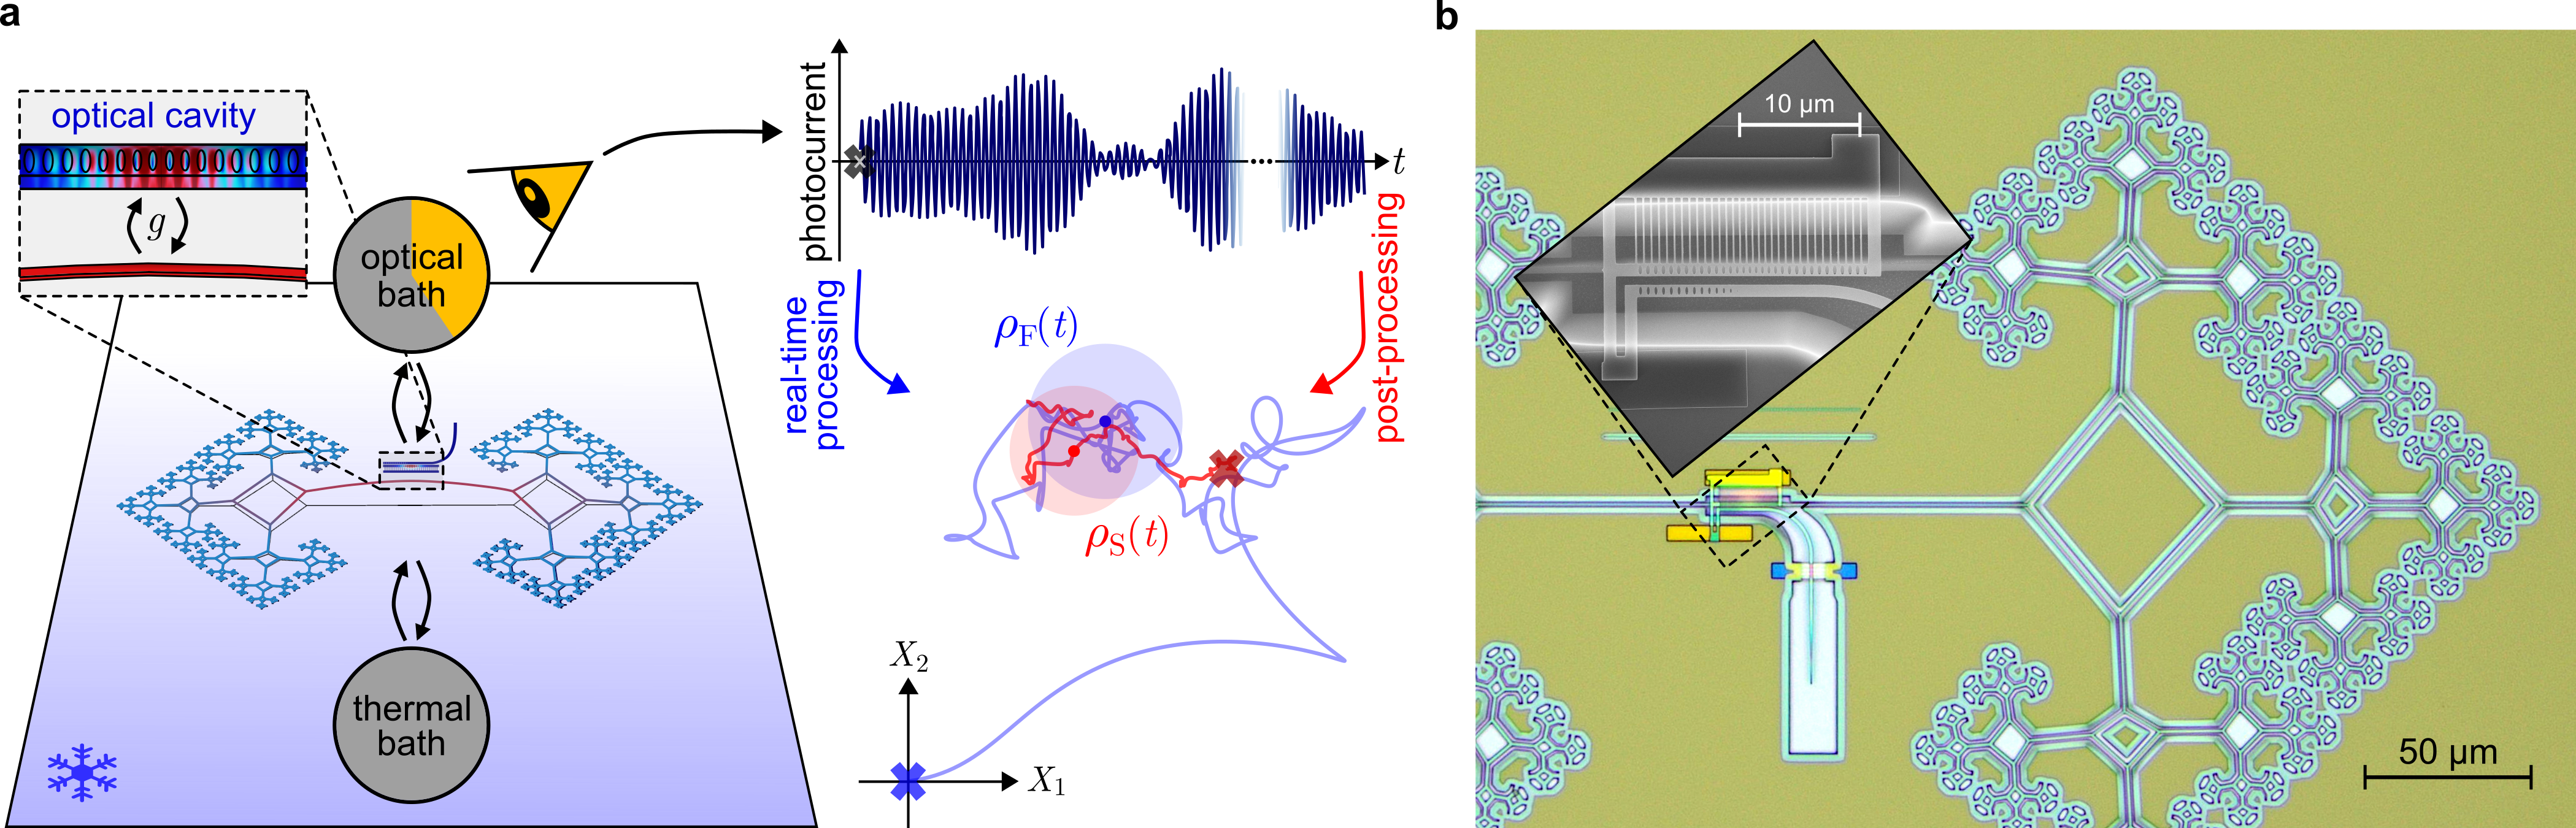
\includegraphics[ ]{FigSetup.png}
    \caption{\textbf{Post-processed quantum trajectories in experiment. a,} A high-quality mechanical resonator, formed by the out-of-plane mode of a hierarchical arrangement of stressed silicon nitride strings, is in contact with a cryogenic thermal bath. It is also in contact with an optical bath, via a photonic crystal cavity coupled with rate $g$. A fraction $\eta$ (yellow) of the optical bath is observed, and the acquired photocurrent is processed to reconstruct the resonator's quantum trajectory. Trajectories obtained from real-time (blue) and post-processed (red) analysis of a sample measurement record diffuse in the rotating phase space spanned by mechanical quadratures $X_{1,2}$. Their means start at distant points (crosses), while their final values coincide. At intermediate time $t$, variances of the inferred Gaussian quantum states are indicated (circles), illustrating that the post-processed state $\rho_{\sm}(t)$ is purer, with smaller variance, than the real-time filtered state $\rho_{\fil}(t)$. \textbf{b,} Optical image of the large optomechanical device, with vertically stacked optical cavity and tapered waveguide for fibre coupling. A scanning electron micrograph (inset) shows the cavity's and waveguide mirror's photonic crystal design.}
    \label{FigSetup}
\end{figure*}

$\rho\fil(t)$  is the optimal real-time estimate of $\rho\fil^\text{LTL}(t)$ (Methods~\ref{sec:QSSforLTL}). As such, the estimate can only be improved, and valuable early-time information recovered, by employing future information and post-processing.
%Recovering the valuable early-time information requires improving upon the optimal real-time estimate of $\rho\fil^\text{LTL}(t)$, which is $\rho\fil(t)$ (Methods), through post-processing of the measurement record. 
To do so, we adapt the quantum state smoothing formalism originally developed for a different scenario --- where two observers, Alice and Bob, simultaneously measure distinct baths interacting with the quantum system~\cite{guevara2015quantum,CGW19} --- and tested very recently in that context~\cite{Shota25}. We reformulate the problem to a sequential scenario so it can be applied to estimate the trajectory of the LTL filtered state. Specifically, the two observers measure the same bath in the same way, with Bob monitoring from the distant past until time $t=0$ and Alice from $t=0$ onwards, while Bob retains access to Alice's record. The task is for Alice to optimally estimate, using only her own record, Bob’s inference, $\rho_{\rm F}^{\rm LTL}(t)$, of the system’s quantum state. Here, the optimal estimate is the $\rho_{\rm C}$ that minimizes the squared Hilbert-Schmidt distance, $\Delta^2_\text{HS}[\rho_\text{F}^\text{LTL},\rho_\text{C}]=\text{Tr}[(\rho_\text{F}^\text{LTL}-\rho_\text{C})^2]$. The relative entropy --- another measure of distinguishability between quantum states --- gives the same optimum~\cite{LGW21}.

The above idea can be applied to general quantum systems (Methods~\ref{sec:QSSforLTL}), but for our experiment we can use the formalism of linear-Gaussian quantum (LGQ) systems~\cite{laverick2019quantum}. 
%\skh{I think this sentence will, most likely, convey that Eq.~(1) is a repetition. What about:} {\color{orange}. The above idea can be applied to general quantum systems (Methods Section~\ref{sec:QSSforLTL}). Adapting the techniques of Ref.~\cite{laverick2019quantum}, we find closed [[or a better word]] formulas for linear-Gaussian quantum systems (as the one that we experiment). Such systems are characterised by ...} 
A LGQ system is characterised by the first and second moments of its phase-space operators. Here we generalise the derivation in Ref.~\cite{laverick2021linear} to obtain the equations for these moments for our smoothed estimate of the LTL filtered state:
%\rep{is characterized by:}{these obey}
%Although each observer knows the other’s measurement setting, only Bob has access to both measurement records. The task is then for Alice to optimally estimate Bob’s inference of the system’s quantum state using only her own record. These standard quantum state smoothing assumptions can be reformulated to enable optimal estimation of the LTL filtered state.
%In the adapted formulation, the two observers measure the same bath in the same way, with Bob monitoring from the distant past until time $t=0$ and Alice from $t=0$ onwards. This mapping allows us to obtain the optimal post-processed (smoothed) estimate of $\rho\fil^\text{LTL}(t)$ by adapting the approach of Refs.~\cite{guevara2015quantum,laverick2019quantum,CGLW21}. We do this for a general quantum system in Methods Section~\ref{?}. For a linear–Gaussian quantum system, the estimate is characterized by (Methods Section~\ref{sec:QSSforLTL}):
\begin{align}
\begin{aligned}
    \langle\hat{\mathbf{x}}\rangle\sm(t) & = \big(\mathbf{V}\sm(t)-\mathbf{V}\fil^\text{ss}\big)\biggl[
    \big(\mathbf{V}\fil(t)-\mathbf{V}\fil^\text{ss}\big)^{-1} \langle\hat{\mathbf{x}}\rangle\fil(t) \\
    &\hspace{5em}+ \big(\mathbf{V}\rfil(t)+\mathbf{V}\fil^\text{ss}\big)^{-1} \langle\hat{\mathbf{x}}\rangle\rfil(t)\biggr]\,, \\
    \mathbf{V}\sm(t) & = \biggl[\big(\mathbf{V}\fil(t)-\mathbf{V}\fil^\text{ss}\big)^{-1}+\big(\mathbf{V}\rfil(t)+\mathbf{V}\fil^\text{ss}\big)^{-1}\biggr]^{-1}\\
    &+\mathbf{V}\fil^\text{ss}\,.
    \label{QSSforLTLfil}
\end{aligned}
\end{align} 
Here, the vector $\hat{\mathbf{x}} = (\hat{q}_1,\hat{p}_1,...,\hat{q}_N,\hat{p}_N)^\text{T}$ contains the canonical operators for position $\hat{q}_j$ and momentum $\hat{p}_j$ of the $N$ system modes, while $\langle\hat{\mathbf{x}}\rangle_\text{C}$ and $\mathbf{V}_\text{C}$ are the mean and covariance matrix of Gaussian Wigner functions inferred from the measurement record, with subscript $\text{C}$ specifying types of conditioning: $\text{F}$ for filtered state (inferred from past measurement data); $\text{R}$ for retrofiltered effect operator (inferred from future data); and $\text{S}$ for smoothed quantum state (inferred from the whole record). Equations for the filtered and retrofiltered moments, derived from the system's stochastic master equation~\cite{laverick2021linear}, are provided in Methods~\ref{sec:GeneralACDK}. 
%\jjs{Maybe a flavour of where they come from? Stochastic master equation?}\ktl{Do you want the SMEs in there? we do cite in the methods the papers that do this in detail.}\jjs{No, not quite, I meant to just give people an idea; suggestion inserted}\ktl{That fine, but we probably need to have a citation here at least}
Finally, $\mathbf{V}\fil^\text{ss}$ is the deterministic covariance matrix of the LTL filtered state, which equals $\mathbf{V}\fil(t)$ in the steady state ($t \to \infty$). %The optimal estimate characterised by $\langle\hat{\mathbf{x}}\rangle\sm$ and $\mathbf{V}\sm$ 
%From Eq.~\eqref{QSSforLTLfil}, we recognize that the mean value $\langle\hat{\mathbf{x}}\rangle\sm$ of the smoothed state is a weighted sum of the stochastic filtered and retrofiltered means $\langle\hat{\mathbf{x}}\rangle\fil$ and $\langle\hat{\mathbf{x}}\rangle\rfil$, respectively, with weights determined by the three covariance matrices $\mathbf{V}\fil$, $\mathbf{V}\rfil$ and $\mathbf{V}\fil^\text{ss}$. These deterministic matrices also directly define the second moment $\mathbf{V}\sm$ of the smoothed state. Moreover,
Eq.~\eqref{QSSforLTLfil} indicates that the smoothed trajectory converges asymptotically to the filtered trajectory after the transient phase, i.e., once $\mathbf{V}\fil(t)\to\mathbf{V}\fil^\text{ss}$. 
%For non-linear Gaussian quantum systems, the smoothing process is conceptually similar but mathematically more involved, as it generally requires numerically generating many realizations of the target quantum trajectories (Methods).

%\jjs{JJS: I was wondering whether a quick nod here to classical smoothing is nice, to indicate that quantum smoothing is importantly different and to foreshadow the shortcomings of the classical formalism. Suggestion below, exact content also depends on what we put in intro}
%{\fgn For filtering, a single procedure---the Kalman-Bucy filter---applies equally to classical and quantum linear Gaussian systems. This is not the case for smoothing. Naively applying the classical approach to a quantum system yields a Gaussian function that follows the structure of Eq.~\eqref{QSSforLTLfil}, but with the target variance $\mathbf{V}\fil\stst$ set to zero. This reflects the classical assumption of a definite underlying value, whereas quantum smoothing correctly accounts for the intrinsic uncertainty of the target state. We revisit the implications of this distinction in more detail later.}

\subsection*{Strong optical monitoring of a  nanomechanical resonator}
%\jjs{Need to check significant figures for quoted values throughout}

The benefits of quantum state smoothing are most pronounced when a substantial fraction of the information leaking from the system into its environment is collected, so that its time evolution can be inferred with near-ground-state resolution.
%\skh{I wonder if we are messing with the concepts that are critical to the paper, like `measuring' the `bath'} {\color{blue} \bf [WPB: is the point that we talk about leaking to the environment' whthout mentioning that the information is going through the bath first? I do like the motivation here. I was wondering whether, somewhere, we need to add a very clear statement on system-bath-environment. Something like "We consider a system that is coupled to one or many baths, such as an optical field or travelling acoustic mode. Some fraction of the based are collected and measured by the observed, while the remainder dissipates into the environment of the system". Alternatively, we could clearly explain what the bath and environment are in our experiments.]}
Notably, in such cases, there is significant back-action associated with the bath under observation itself. 
% \skh{I don't know; the amount of back-action is not about how much info is collected---I know I suggested `collected', but it doesn't work}\jjs{I tried to get around that by specifying `bath under observation'; its (relative) back-action does put a limit on how much info \emph{can be} collected, right?}\skh{much better; maybe all good for me} 
Cavity optomechanical systems --- where an optical probe enables quantum-limited readout of mechanical motion --- offer an important platform for achieving this regime~\cite{aspelmeyer2014cavity,mason2019continuous,rossi2019observing,bowen2015quantum}. Moreover, tracking the trajectory of a macroscopic resonator underpins applications in quantum control~\cite{guo2019feedback}, gravitational wave and dark matter detection~\cite{muller2008entanglement,hirschel2024superfluid,baker2024optomechanical}, and proposed tests of quantum gravity~\cite{girdhar2020testing}. 

To validate our approach and demonstrate the utility of quantum state smoothing in experiment, 
we track the quantum trajectory of the fundamental out-of-plane resonance of
%a mechanical resonator that is coupled a mechanical thermal bath and an optical bath. Combined with 
the on-chip mechanical structure shown in FIG.~\ref{FigSetup}, which has a frequency of $\Omega/2\pi = 1.04$~MHz. 
%This out-of-plane {\color{blue} resonance has a} resonance frequency of $\Omega/2\pi = 1.04$~MHz and
%constitutes a single-mode linear Gaussian system.
%\skh{Not here probably because being a `linear Gaussian' system is a combinational effect of the resonator's Hamiltonian, it's interaction with the optical bath and the homodyne measurement on the optical bath} 
%\jjs{That's fair; couldn't find the optimal place yet. Will think about later.}
We monitor this resonance via dispersive coupling to a telecom-wavelength photonic crystal cavity with linewidth $\kappa/2\pi=11.5$~GHz (Methods~\ref{sec:methods:char_optical}).
The combined optomechanical system is well inside the fast-cavity limit, so that the cavity dynamics can be adiabatically eliminated.
Consequently, the mechanical displacement is directly imprinted on the phase of a resonant laser probe reflected off the cavity~\cite{bowen2015quantum}, which we detect with efficiency $\eta$ using shot-noise-limited homodyne measurement (Methods~\ref{SecHomoSetup}).

As illustrated in FIG.~\ref{FigSetup}\textbf{a}, the cavity mediates an interaction between the resonator and an optical bath. The rate at which information leaks into 
% \skh{at which it interacts with??}\jjs{I like the information focus, hoped it wasn't too contentious ;)}\skh{I'm not sure really how contentious it is; but to the least, shouldn't it be `info is leaking'?} 
the optical bath is given by $\gamma_\text{opt} = 4\bar{n}_\text{cav} g_0^2/\kappa$, where $g_0$ is the single-photon optomechanical coupling rate and $\bar{n}_\text{cav}$ the mean cavity photon number~\cite{bowen2015quantum,meng2020mechanical}. At the same time, information leaks into the resonator's mechanical thermal bath at a rate $\gamma_\text{th}$. In the limit that the resonator temperature $T \gg \hbar \Omega/k_\text{B}$, relevant to our experiments, this is approximated as $\gamma_\text{th} \approx \Gamma n_\text{th}$~\cite{aspelmeyer2014cavity}, where $\Gamma$ is the resonator's energy decay rate and $n_\text{th}\approx k_\text{B} T/(\hbar \Omega)$ its thermal occupancy. %\skh{By being too explicit here, we are running into troubles. What Jesse had initially written was `fluctuation exchange at the rate $\Gamma n_\text{th}$' and I said `we cannot say ``exchange" of fluctuations at this rate because of figure 6 in~\cite{aspelmeyer2014cavity}'. What we now call the `rate of leaking info', seems to be exactly $\Gamma n_\text{th}$ (Methods~\ref{SecFullHete}).}
%at temperature $T$~\cite{aspelmeyer2014cavity}.  
With these bath interactions and the homodyne measurement, the resonator constitutes a single-mode linear Gaussian system.
%the resonator receives fluctuations from its thermal environment at a rate $\gamma_\text{th} = \Gamma n_\text{th}$, where $\Gamma$ is the energy decay rate of the mechanical resonator and $n_\text{th}\sim k_B T/(\hbar \Omega)$ \skh{or $k_\text{B}$ ?} is the occupancy of its thermal phonon bath at temperature $T$. 
%\jjs{There's a subtlety here: strictly speaking, information leaks into the mechanical thermal bath at rate $\gamma_\text{th} = \Gamma (n_\text{th} + 1)$ (see e.g. Aspelmeyer 2014, Fig. 6). That's why previous version mentioned `fluctuations enter' at rate $\Gamma n_\text{th}$ instead (cf. same figure). Is the most correct thing: keep the new version and change the ratio to $\gamma_\text{opt} / \gamma_\text{th} = \mathcal{C}/(n_\text{th} + 1)$? Also indicates that even at zero temperature, $\mathcal{C} > 1$ is what you want.} {\color{blue} \bf [I think it was important to be talking about information for both baths, rather than switching between information and fluctuations. Happy to add the +1 if you like, also should include a cite the aspelmeyer paper. I do note that the approximation of neglecting the plus one is consistent with our approximation for $n_{th}$. Either way, should cite Aspelmeyer to justify.]}

As only the detected part of the optical bath can be accessed, to effectively monitor the system one must maximize both the optical detection efficiency $\eta$ and
the ratio $\gamma_\text{opt}/\gamma_\text{th} = \mathcal{C} / n_\text{th}$, where $\mathcal{C} = 4\bar{n}_\text{cav} g_0^2 / (\kappa \Gamma)$ is the optomechanical cooperativity.
Our optomechanical device is carefully engineered to do this~\cite{guo2022integrated,guo2023active}.
Acoustic clamping losses are minimized by the resonator's hierarchical fractal structure~\cite{fedorov2020fractal},
%\jjs{Still need to check role of dissipation dilution: reduce $\Gamma$ or increase $\Omega$?}
resulting in an exceedingly low decay rate of $\Gamma/2\pi = 11.5$~mHz at cryogenic temperatures (Methods~\ref{sec:methods:char_mechanical}).
Simultaneously, vertical integration of the optical cavity allows for a large single-photon optomechanical coupling rate of $g_0/2\pi = 159~$kHz (Methods~\ref{sec:methods:char_coupling}). 
% \jjs{Stiffening tethers shift the mechanical modes of the cavity structure itself to higher frequencies.} \skh{No need for this, I would say}
Details on device structure and fabrication are discussed in Ref.~\cite{guo2022integrated}.

The device is placed in a dilution refrigerator to reduce $n_\text{th}$.
%\jjs{I removed the mK base temperature, because we don't run at base temp. Alternatively, could add: ``While currently operated at $T = 3.6$~K, this allows for future experiments in the mK regime.''?}
We drive the cavity to a mean photon number of $\bar{n}_\text{cav} = 41.4$ ($\mathcal{C} = 3.16 \times 10^4$), limited by higher frequency mechanical resonances that introduce coloured noise at larger $\bar{n}_\text{cav}$. Optical absorption raises resonator temperature to $T=12.1$~K (Methods~\ref{sec:methods:mode_temperature}), so that $n_\text{th} = 2.45 \times 10^5$ and $\mathcal{C}/n_\text{th} = \gamma_\text{opt}/\gamma_\text{th} \approx 0.13$ -- indicating that an appreciable fraction of information enters the optical bath.

%(Methods Section~\ref{?}) 
At the mean cavity photon number used,
%Even at this photon number, 
we find that the mechanical resonator intermittently switches to a self-oscillating regime.
We suppress this instability by applying weak, phase-tuned, band-limited optical feedback (Methods~\ref{sec:methods:setup_feedback})
%~\cite{Purdy2013observation}
, which is effectively Markovian and increases the effective mechanical decay rate to $\Gamma_\text{fb}/2\pi = 85$~Hz. 
While the feedback could, in principle, be modelled explicitly within the system dynamics, in our case it suffices to replace $\Gamma\to\Gamma_\text{fb}$ and $n_\text{th}\to n_\text{th}\times\Gamma/\Gamma_\text{fb}$ in analysis (Methods~\ref{SecFeedbackModelling}). 
% This leaves the cooperativity ratio $\mathcal{C}/n_\text{th}$ unchanged~\cite{Purdy2013observation}.
This leaves the ratio $\gamma_\text{opt}/\gamma_\text{th}$, unchanged.
% \skh{this sentence doesn't need a citation as it is simple math; right? Could you please also read the feedback modeling section in Methods-Analysis? just to make sure that you've captured the story here.} \jjs{The citation points to a classic paper where the same strategy was used, could move it to a different spot. Also, added a bit more detail; better?}\skh{great to have a classical citation for the replacement approach, but I believe it should move.}\jjs{Moved}

%\skh{Why is it mentioned after the feedback replacement $n_\text{th}\to n_\text{th}\times\Gamma/\Gamma_\text{fb}$? This will be super confusing.}
%indicating that the strength of interaction with the optical bath is comparable to that with the thermal bath.
%This results in a ratio of optical to thermal bath coupling rates of $\gamma_\text{opt}/\gamma_\text{th} = \unsure{0.131}$, indicating that the strength of interaction with the optical bath is comparable to that with the thermal bath.

To maximise $\eta$, the cavity is first evanescently coupled 
% \skh{could this be in passive tone instead?}
to an on-chip waveguide with efficiency $\eta_\text{esc} = 0.82$. The waveguide's shape is engineered to maximize transfer to a
complementarily tapered optical fibre. 
After cool-down, we carefully optimize the fibre–waveguide alignment inside the dilution refrigerator to achieve a notably high transfer efficiency of $\eta_\text{wf} = 0.77$ (Methods~\ref{sec:methods:optical_coupling}).
% After cool-down, we optimize the fibre–waveguide alignment inside the dilution refrigerator by imaging it with an external microscope, achieving a notably high transfer efficiency of $\eta_\text{wf} = 0.77$ (Methods).
% Notably, we optimize the fibre-waveguide alignment inside the dilution refrigator after cool-down, imaging the alignment with an outside microscope, to attain a high transfer efficiency $\eta_\text{wf} = 0.77$ (Methods).
Minimizing inefficiencies in the optical fibre path and employing high-efficiency, low-noise photodiodes, we achieve a total efficiency of $\eta = 0.38$, verified independently using a new method that exploits the mechanical instability (Methods~\ref{sec:methods:eta_check}). 
Together with our high ratio of optical to thermal bath coupling, this allows us to track the resonator's evolution in real-time with a resolution about $4.7$ times higher than its zero point motion, indicating that quantum backaction will play a significant role in the system dynamics. 
Validating this, we demonstrate ponderomotive squeezing of light by quantum backaction~\cite{bowen2015quantum} (Methods~\ref{sec:methods:mode_temperature}).

\subsection*{Experimental estimation of the long-time-limit filtered state}

To determine the resonator’s filtered and smoothed trajectories ($\rho_\text{F}$ and $\rho_\text{S}$), and statistically compare them with its LTL filtered trajectory ($\rho_\text{F}^\text{LTL}$), we monitor the nanomechanical resonator for several seconds and record the homodyne photocurrent.  
%{\color{blue} These photocurrents are processed to obtain $\langle\hat{\mathbf{x}}\rangle_\text{F}$, $\langle\hat{\mathbf{x}}\rangle_\text{R}$, $\mathbf{V}_\text{F}$ and $\mathbf{V}_\text{R}$, which define $\rho_\text{F}$ and also provide input to Eq.~\eqref{QSSforLTLfil} to obtain $\rho_\text{S}$.
%
%using the filtering and retrofiltering equations given in the Methods (Eqs.~\eqref{?} and \eqref{?}) to obtain trajectories of the mean values $\langle\hat{X}_j\rangle_\text{F}$ and $\langle\hat{X}_j\rangle_\text{R}$, where $j \in \{1,2\}$. 
%
% For each record,
%We then divide the measurement time into $750$-µs intervals. For each interval,
% 
The photocurrent is normalized to the shot noise level and demodulated at mechanical frequency $\Omega$. This neglects the fast-oscillating dynamics of the resonator while retaining the effective interaction-frame dynamics~\cite{doherty2012quantum}. The demodulation produces two measurement currents corresponding to heterodyne detection of the resonator’s quadratures, $\hat X_{1}=\cos(\Omega t)\,\hat q-\sin(\Omega t)\,\hat p$ and $\hat X_{2}=\sin(\Omega t)\,\hat q+\cos(\Omega t)\,\hat p$, where the mechanical position $\hat{q}$ and momentum $\hat{p}$ are normalized to have ground-state variance of one. We divide these quadrature currents into 16,653 750-$\mu$s-long measurement records. 

The measurement records are processed using the filtering and retrofiltering equations given in Methods (Eqs.~\eqref{equ:rFT} and \eqref{equ:rRT}) to obtain trajectories of the mean values $\langle\hat{X}_j\rangle_\text{F}$ and $\langle\hat{X}_j\rangle_\text{R}$, where $j \in \{1,2\}$. The trajectories of the covariances, $\mathbf{V}_\text{F}$ and $\mathbf{V}_\text{R}$, are deterministic and set by the experimental parameters $\Gamma$, $\mathcal{C}$, $n_\text{th}$, and $\eta$ (Eqs.~\eqref{VFT} and \eqref{VRT}). Together, $\langle\hat{X}_j\rangle_\text{F}$ and $\mathbf{V}_\text{F}$ provide the filtered quantum state trajectory. The smoothed quantum state trajectory is obtained by introducing $\hat{\mathbf{x}}=(\hat{X}_1,\hat{X}_2)^\text{T}$ with the moments calculated by filtering and retrofiltering
into Eq.~\eqref{QSSforLTLfil}. Finally, the LTL filtered trajectory is determined similar to the filtered trajectory, but with the filtering interval extended over the three preceding records. This ensures that the filtering covariance matrix converges to $\mathbf{V}_\text{F}^\text{ss}$, as the transient phase lasts for about half a record.
\begin{SCfigure*}
    \centering 
    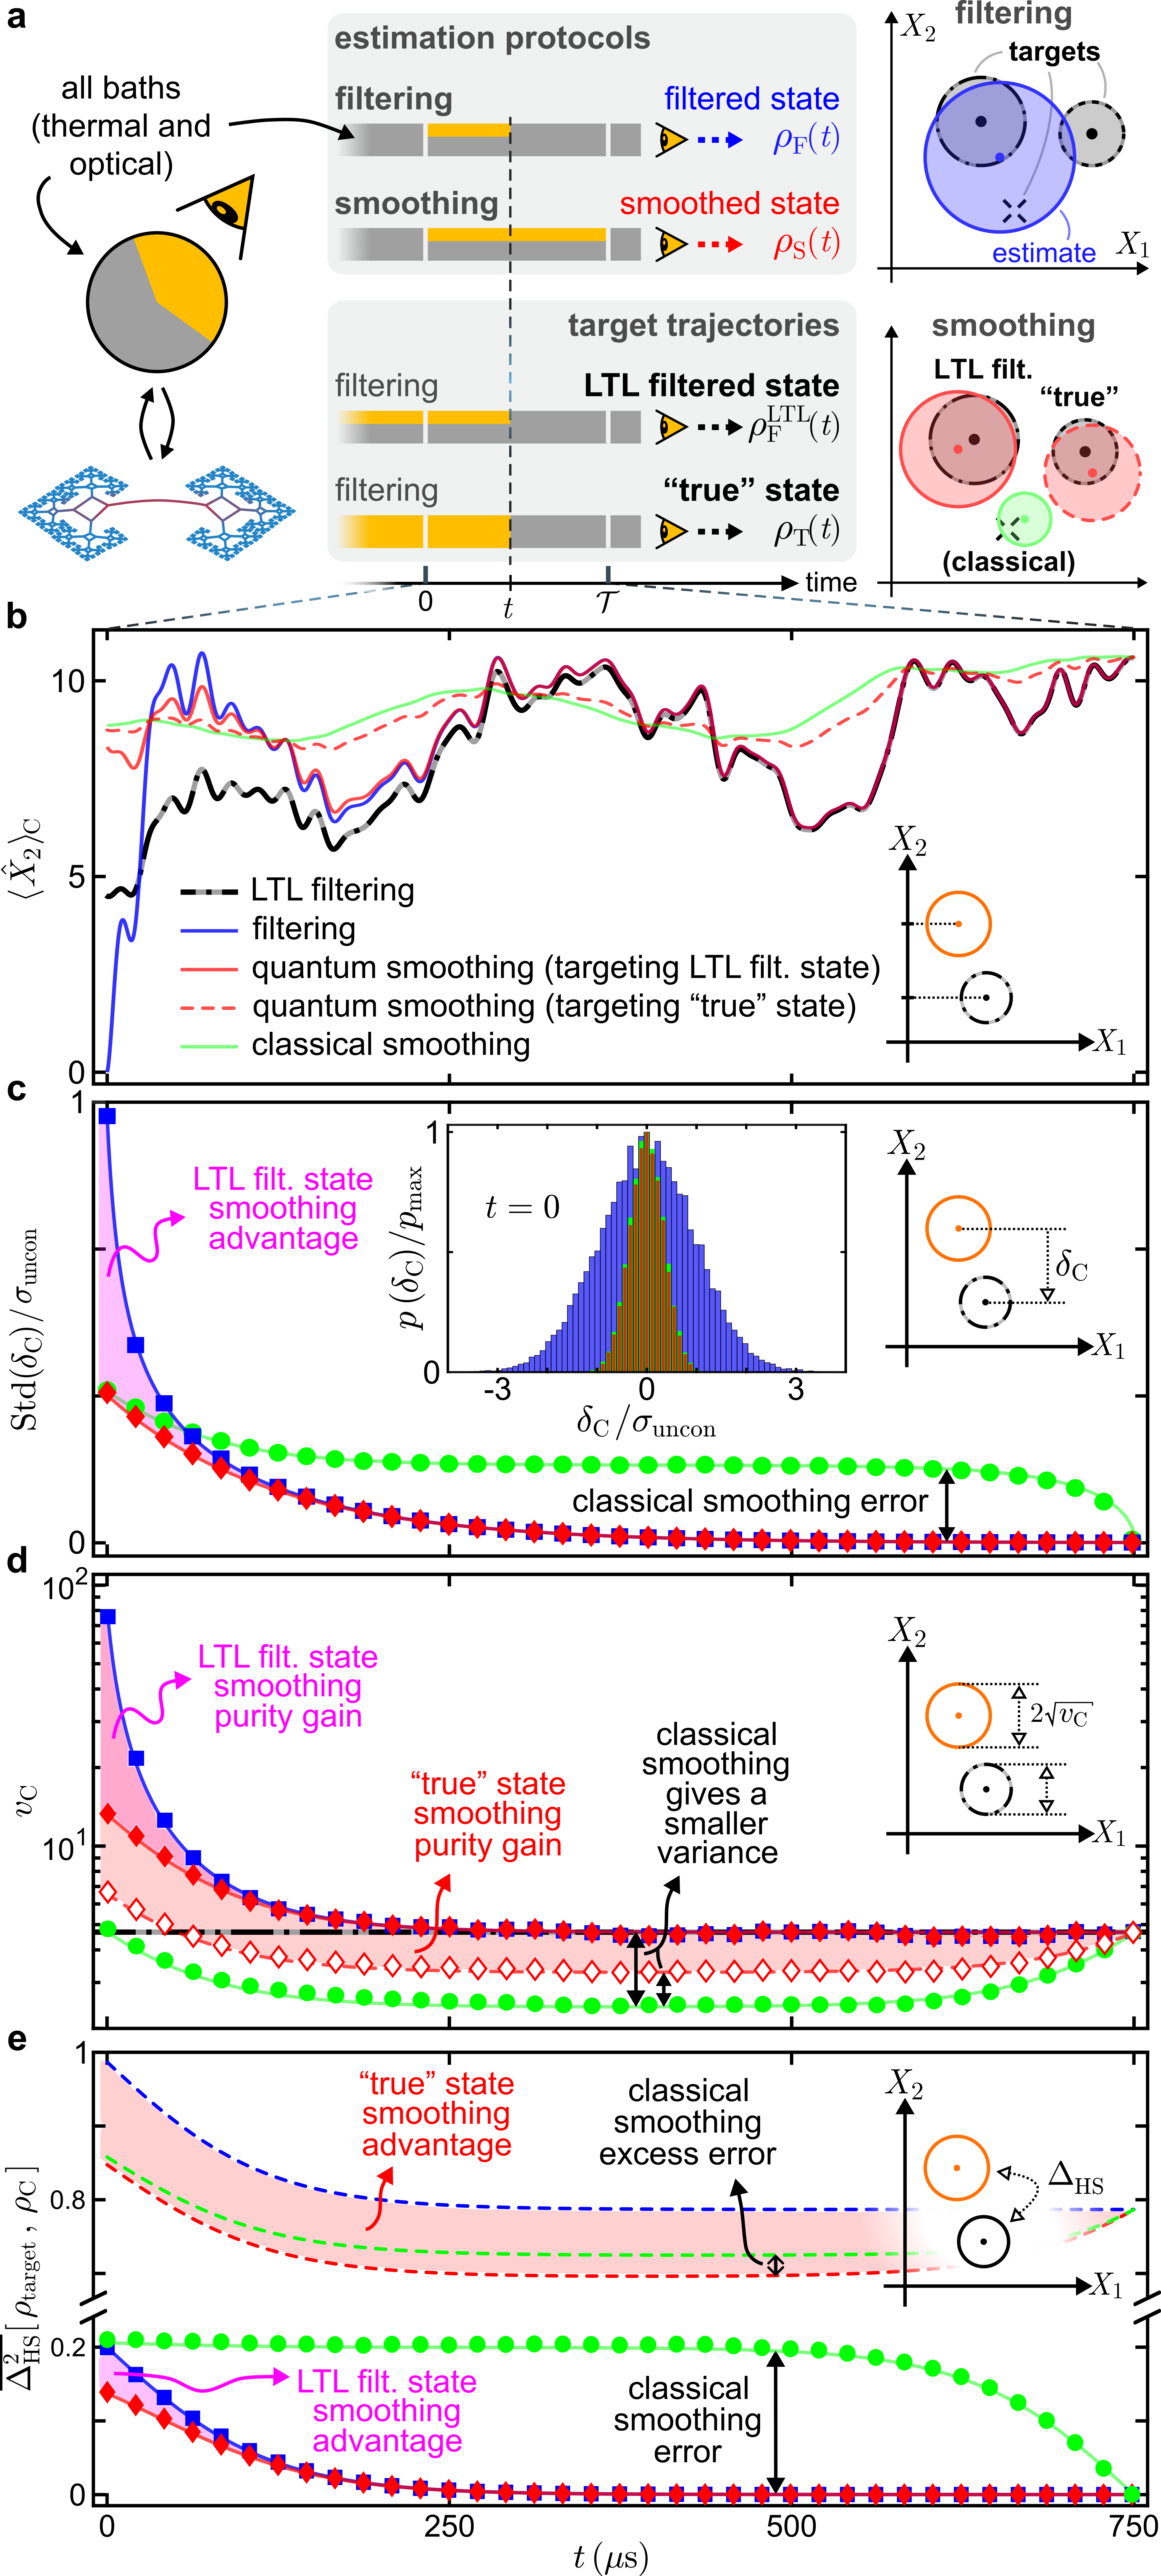
\includegraphics[width=\linewidth]{FigData1.png}
    \caption{\textbf{Inferred trajectories of the mechanical resonator. a,} Conceptual illustration of the inference process.
    Each bar represents all the baths as a whole that continuously interacts with the resonator. The yellow portions indicate the extent to which this combined bath is measured over time, with the outputs used to infer a quantum state for the resonator at record time $t$ (dashed line). Estimator states are inferred from the actual measurement record --- either from $0$ to $t$ (filtered state) or from $0$ to the record end $\mathcal{T}$ (smoothed state) --- whereas target trajectories assume access to a long-time-limit (LTL) measurement history and to all baths (``true"). As illustrated in phase space (right), both target trajectories share a single real-time estimator ($\rho_{\fil}$, blue) but differ in their optimal post-processed estimators ($\rho_{\sm}\text{'s}$, red). The filtered state $\rho_{\fil}$ also provides the optimal estimate of the fictitious true value (cross) of the resonator’s classical counterpart, which has its own post-processed estimator (green).
    \textbf{b-e,} Comparing the estimation protocols. Insets on the right indicate the quantity plotted in each panel, as computed from estimator (orange) and target (black) states.
    \textbf{b,} Stochastic traces of the quadrature mean $\langle\hat{X}_2\rangle(t)$ for a sample measurement record.
    \textbf{c,} Standard deviation of distance $\delta_\text{C}(t)=\langle\hat{X}_j\rangle_\text{F}^\text{LTL}(t)-\langle\hat{X}_j\rangle_\text{C}(t),\,j=1,2$ between the LTL target and its estimators (C = F, S) or the classical smoother (C = cS), normalised to the unconditional state size $\sigma_\text{uncon}$. Statistics derived from an ensemble of 16,653 records (data points) correspond well to theory (lines). Inset histogram shows the distributions of $\delta_\text{C}(0)$ across the ensemble.
    \textbf{d,} Deterministic variances $v_\text{C}$ of the estimator states, of the classical smoother and of the LTL target. Estimators' variances agree well with the corresponding value of $\sigma^2_\text{uncon}-\mathbb{V}\mathrm{ar}_{\text{ens}}[\langle\hat{X}_j\rangle_\text{C}(t)]$, calculated across the ensemble of records (data points, Supplementary~\ref{SecConsistency} and \ref{sec:ErrorBars_forSC}).
    \textbf{e,} Distinguishability of the estimator states from their corresponding targets, and of the classical smoother from both quantum targets. The measure is the estimation cost function, given by the ensemble-averaged Hilbert-Schmidt distance squared, $\Delta^2_\text{HS}[\,\rho_\text{target}(t)\,,\,\rho_\text{C}(t)]=\text{Tr}[(\rho_\text{target}(t)-\rho_\text{C}(t))^2]$. Theory (lines) and experimental values (data points) are shown.}
    \label{FigData1}
\end{SCfigure*}

The outputs of the analysis are shown in FIG.~\ref{FigData1}. The schematic in FIG.~\ref{FigData1}\textbf{a} summarizes the two estimation protocols and their target, $\rho_\text{F}^\text{LTL}(t)$. Filtering uses the record data from time zero until the present time $t$. Smoothing uses the entire record, combining filtering of past data (between zero and $t$) with retrofiltering of future data (between $t$ and $750~\mu$s). FIGs.~\ref{FigData1}\textbf{b–e} compare the trajectories, each defined by the mean values $\langle \hat{X}_1\rangle$ and $\langle \hat{X}_2\rangle$ (for brevity, only $\langle \hat{X}_2\rangle$ is shown; $\langle \hat{X}_1\rangle$ is presented in Supplementary~\ref{sec:DataForX1}), together with
a single parameter $v$ that fully specifies the covariance matrix ($\mathbf{V}=v\,\mathbf{I}$, with $\mathbf{I}$ the $2\times 2$ identity matrix). This single-parameter description of $\mathbf{V}$ is possible due to the 
dynamical symmetry of $\hat X_{1}$ and $\hat X_{2}$ when $\Omega\gg\gamma_{\rm opt},\gamma_{\rm th}$~\cite{doherty2012quantum}.

FIG.~\ref{FigData1}\textbf{b} shows $\langle\hat{X}_2\rangle$ for a sample measurement record. For filtering (blue), it starts at zero --- the unconditional mean --- well separated from the LTL target value (dashed black). For smoothing (solid red), it begins closer to the target, as smoothing incorporates future data. The two estimates converge in the second half of the record interval. To statistically assess the accuracy of these estimates, we calculate the distance $\delta_\text{C}(t)=\langle\hat{X}_j\rangle_\text{F}^\text{LTL}(t)-\langle\hat{X}_j\rangle_\text{C}(t)$ for filtering ($\text{C}=\text{F}$) and smoothing ($\text{C}=\text{S}$) across the ensemble of records. The standard deviation of $\delta_\text{C}$ is shown in FIG.~\ref{FigData1}\textbf{c}. At $t=0$, it is smaller for smoothing (red) than for filtering (blue) by a factor of three, and it remains smaller throughout the transient phase, demonstrating the advantage of smoothing.

FIG.~\ref{FigData1}\textbf{d} shows the deterministic conditional variances. In the transient phase, $v_\text{S}$ (solid red) is smaller than $v_\text{F}$ (blue), indicating that the smoothed state is purer than the filtered state as purity is given by $1/\sqrt{\det[\mathbf{V}_\text{C}]} = 1/v_\text{C}$~\cite{serafini2017quantum}. Specifically, the smoothed state is about six times purer at $t=0$. While these variances cannot be directly measured --- a set of projective measurements evaluating $v_\text{F}$ would disturb the resonator’s dynamics --- they are involved in the inference of $\langle\hat{X}_j\rangle_\text{C}$ (Methods~\ref{SME-ME-&Analysis}) and are thus linked to the experimental mean-value traces. Provided the system is accurately modelled and characterised, and the measurement data properly analysed, $v_\text{C}(t)$ equals the variance difference $\sigma^2_\text{uncon}-\mathbb{V}\mathrm{ar}_{\text{ens}}[\langle\hat{X}_j\rangle_\text{C}(t)]$, where $\sigma^2_\text{uncon}$ is the unconditional variance and the last term is evaluated over a sufficiently large ensemble of measurement records (Supplementary~\ref{SecConsistency}). We test this inference consistency by calculating the variance difference from the collected ensemble (solid red diamonds and blue squares in FIG.~\ref{FigData1}\textbf{d}). The close agreement with $v_\text{C}(t)$ confirms the reliability of our analysis.
%\jjs{From Eq.~\eqref{QSSforLTLfil} and the condition $v\fil^{\rm ss} \approx v_{\rm R}^{\rm ss}$ it can be seen that, generally, $v\sm(0) = 3 v_{\rm LTL} = 3 v\fil^{\rm ss}$. i.e. factor 3 is not a coincidence. Comment worthy?} 

Finally, the accuracy of the estimator state trajectories is assessed by calculating the ensemble-averaged squared Hilbert–Schmidt distance. The data points in FIG.~\ref{FigData1}\textbf{e} show the experimentally measured values, in close agreement with the theoretical curves. At $t=0$, the measured value for smoothing (solid red diamond) is roughly two-thirds of that for filtering (blue square), and it remains smaller for smoothing throughout the transient phase. The smoothed state is thus demonstrated to be closer to the target than the filtered state, yielding a more accurate trajectory for the resonator.

% \noindent
% \makebox[0pt][l]{\rule{\linewidth}{0.5pt}}%
% \makebox[\linewidth][r]{\rule{0.5pt}{0.6em}}
% \noindent
% \begin{minipage}{\linewidth}
% \fontsize{9}{10.5}\selectfont
% ... text ...
% \end{minipage}

% \vspace{1.4em}
% \noindent
% \makebox[0pt][l]{\rule{\linewidth}{0.5pt}}%
% \makebox[\linewidth][l]{\raisebox{-0.6em}{\rule{0.5pt}{0.6em}}}
% \noindent

\section{Quantum trajectories of the ``true" state} \label{Sec:true}

Because all real quantum systems interact with baths that are not measured, the LTL filtered state is never pure in practice.
%As in our experiment, monitored quantum systems usually interact with baths that are not measured. Consequently, the LTL filtered state is typically mixed, and 
%{\color{green} {\bf [WPB: I wonder if this sentence is necessary at all --- feels like a repeat of the next one that could be safely deleted]} Its trajectory --- targeted so far in this paper --- is not the most informative description of the system’s evolution available in principle.} 
Were one able to measure the
unobserved baths, or access the outputs of naturally occurring measurements on them, one could produce a more accurate trajectory of the system’s evolution. We refer to the system’s state, conditioned on measurements on all baths far into the past, as the ``true" state $\rho_\text{T}(t)$. Ideally, this state is pure and evolves according to a stochastic Schrödinger equation. The trajectory of the true state, as the
best possible description of the system’s evolution, is our next estimation target.

As with the LTL filtered state, the optimal real-time estimate of $\rho_\text{T}(t)$ is given by the system’s filtered state~\cite{guevara2015quantum}. However, as we show below, a better estimate can be obtained using future data. In previous studies of the quantum state smoothing formalism, Bob and Alice measure their respective baths from time $t=0$ assuming the same initial state \cite{guevara2015quantum,GueWis20,laverick2021quantum,laverick2021linear,CGLW21,LGW21}, with most taking that to be a pure state. Here we generalize this to an impure initial state for Alice by imagining that Bob monitors all baths from the distant past until $t=0$, at which point he hands one bath (or part of a bath) to Alice, who begins measuring it while Bob continues observing the remaining baths as well as having access to Alice's record. For a Gaussian true state, the smoothed estimate is characterised by Eq.~\eqref{QSSforLTLfil}, with $\mathbf{V}_\text{F}^\text{ss}$ replaced by the deterministic covariance matrix of the true state (that is, Bob's state), \blk $\mathbf{V}_\text{T}^\text{ss}$.
%For a non-Gaussian true state, the estimation process is more involved, as outlined in the Methods. 
%in a manner analogous to the LTL filtered state estimation (Methods).

The set of possible true states conditioned, in part, on naturally occurring measurements (on the unobserved baths) depends on the types of interactions between the unobserved baths and the larger environment which acts as a measurement apparatus for those baths. Since these interactions are generally unknown, this set is also not known in general. However, in our case, there is a unique ``unravelling'' (type of measurement) which satisfies the following desiderata for naturalness: (i) the resulting stochastic master equation of the system should be invariant under transformations that preserve the master equation (see Methods~\ref{sec:methods_Nat_Unrav} and Refs.~\cite{gisin1992quantum,gisin1992wave});
and (ii) the measurement should be Markovian, just as the baths are. Under these criteria, the natural unravelling of the resonator’s symmetric master equation is unique and corresponds to heterodyne detection~\cite{WisDio01}. This unravelling on the unobserved baths of course matches with the unravelling on the observed bath, which is another reason it is natural for our system. Considering the total unravelling, the true state of the system is a stochastic coherent state (that is, the ground state with a stochastic phase-space displacement) (Methods~\ref{SecFullHete}).

\subsection*{Experimental ``true" state estimation}

We now estimate the resonator's true trajectory (FIG.~\ref{FigData1}\textbf{a}). Its real-time estimate is the filtered trajectory already characterized by $\langle\hat{X}_{j}\rangle_\text{F}$ and $v_\text{F}$. Its post-processed estimate is given by Eq.~\eqref{QSSforLTLfil}, with all $\mathbf{V}\fil^\text{ss}$ terms replaced by $\mathbf{V}\god^\text{ss}=\mathbf{I}$, the covariance matrix of a displaced ground state, and $\hat{\mathbf{x}}=(\hat{X}_1,\hat{X}_2)^\text{T}$, considering the previously calculated values of $\langle\hat{X}_{j}\rangle_\text{F}$, $\langle\hat{X}_{j}\rangle_\text{R}$, $v_\text{F}$ and $v_\text{R}$. The results are shown in FIG.~\ref{FigData1}. Until the very end of the measurement record, the smoothed estimate differs from both the filtered estimate and from the smoothed estimate of the LTL filtered trajectory. For example, the red dashed line in FIG.~\ref{FigData1}\textbf{b} shows the markedly different value of $\langle\hat{X}_2\rangle_\text{S}$ for the sample record. As the smoothing here targets the true state rather than the LTL filtered state, some dynamics uncorrelated with the LTL state (dashed black) are evident.

%While some correlation with the LTL filtered state (black line) can be observed, a substantial component of uncorrelated dynamics is also evident and the traces do not converge until the very end of the record. This is to be expected, since the smoothing here targets the true state rather than the LTL filtered state.
%by feeding the values of $\langle\hat{X}_{j}\rangle_\text{F}$ and $\langle\hat{X}_{j}\rangle_\text{R}$, together with the deterministic $\mathbf{V}_\text{F}$ and $\mathbf{V}_\text{R}$, into Eq.~\eqref{QSSforLTLfil} with $\hat{\mathbf{x}}=[\hat{X}_1,\hat{X}_2]^\text{T}$ and $\mathbf{V}\fil^\text{ss}$ replaced by $\mathbf{V}\god^\text{ss}=\mathbf{I}$, as the true state is a displaced ground state.  
%where $v_\text{GS}=1$ is the ground state variance.
%The estimation results are shown in FIG. \ref{FigData1}. The real-time estimate (blue line) is unchanged from the previous case where the target was the LTL filtered state trajectory.
%{\color{blue} This is because in} {\cya both the LTL and true state cases, the target states resulted from an valid continuous-in-time unobserved measurement happening on the system. This means that averaging over the unobserved measurement outcome reproduces the dissipation that would have occurred had no measurement been performed. Thus, since in both cases Alice is performing the same measurement with the same efficiency, we obtain the same filtered state.}  {\color{blue}\bf [WPB: is there an intuitive reason?]}. \skh{I don't have one. Do you Kiarn, Howard?}\ktl{KTL: Is this too long? or too detailed? This is the reason though, feel free to edit as you wish.}
%By contrast, the smoothed estimate (red dashed line) is markedly different across the full measurement record. For instance, the dashed red line in FIG.~\ref{FigData1}\textbf{b} shows the smoothed estimate of $\langle\hat{X}_2\rangle_\text{S}$. While some correlations with the same moment of the LTL filtered state (black line) can be observed,
%\skh{SK: are you comparing with LTL itself and not with its smoothed estimate?}
%a substantial component of uncorrelated dynamics is also evident and the traces do not converge until the very end of the record. This is to be expected, since here the smoothing targets the true state rather than the LTL state. 
%The value of $\langle\hat{X}_2\rangle_\text{S}$, for the sample measurement record employed in FIG. \ref{FigData1}\textbf{b}, is plotted with the dashed-red curve. It differs from the filtered value $\langle\hat{X}_2\rangle_\text{F}$ until the end of the record. 

The variance of the smoothed quantum state $v{\sm}$ is shown by the red dashed curve in FIG.~\ref{FigData1}\textbf{d}. It begins below the filtering variance $v{\fil}$ (blue curve) at $t=0$ and remains lower as both gradually decrease until they reach their steady-state values. Near the end of the record, where less future data is available for smoothing, $v{\sm}$ begins to increase towards $v{\fil}$. As $v{\sm}$ is smaller than $v{\fil}$, the smoothed state is purer than the filtered state. Similar to LTL estimation, there is a purity gain in the initial transient phase, exceeding an order of magnitude at $t=0$. In contrast to LTL estimation, the purity gain persists into the steady state, where both $v_\text{S}$ and $v_\text{F}$ have steady values, leaving the smoothed state 43\% purer. The consistency of the inference of this smoothed state is tested by calculating $\sigma^2_\text{uncon}-\mathbb{V}\text{ar}_{\text{ens}} [\langle\hat{X}_j\rangle_\text{S}(t)]$  (hollow red diamonds in FIG.~\ref{FigData1}\textbf{d}), which matches $v{\sm}(t)$ as predicted analytically (Supplementary~\ref{SecConsistency}).
%Analytical derivation (Supplementary Section~\ref{SecConsistency}) shows that the difference should equal $v{\sm}(t)$, and our data is consistent with this prediction (hollow red diamonds, FIG.~\ref{FigData1}\textbf{d}).

The dashed curves in FIG. \ref{FigData1}\textbf{e} show the average value of the estimation cost function $\Delta^2_\text{HS}[\rho_\text{T},\rho_\text{C}]=\text{Tr}[(\rho_\text{T}-\rho_\text{C})^2]$ --- red dashed for $\text{C}=\text{S}$ and blue dashed for $\text{C}=\text{F}$. Throughout the entire record, the smoothed quantum state better estimates the target and thus its trajectory captures the resonator's evolution more accurately. These curves are not accompanied by experimental data because the mean values of the pure true state are inaccessible to our experiment; obtaining them would require access to the unobserved baths or to the information leaking from them into the rest of the environment.
\begin{SCfigure*}
    \centering
    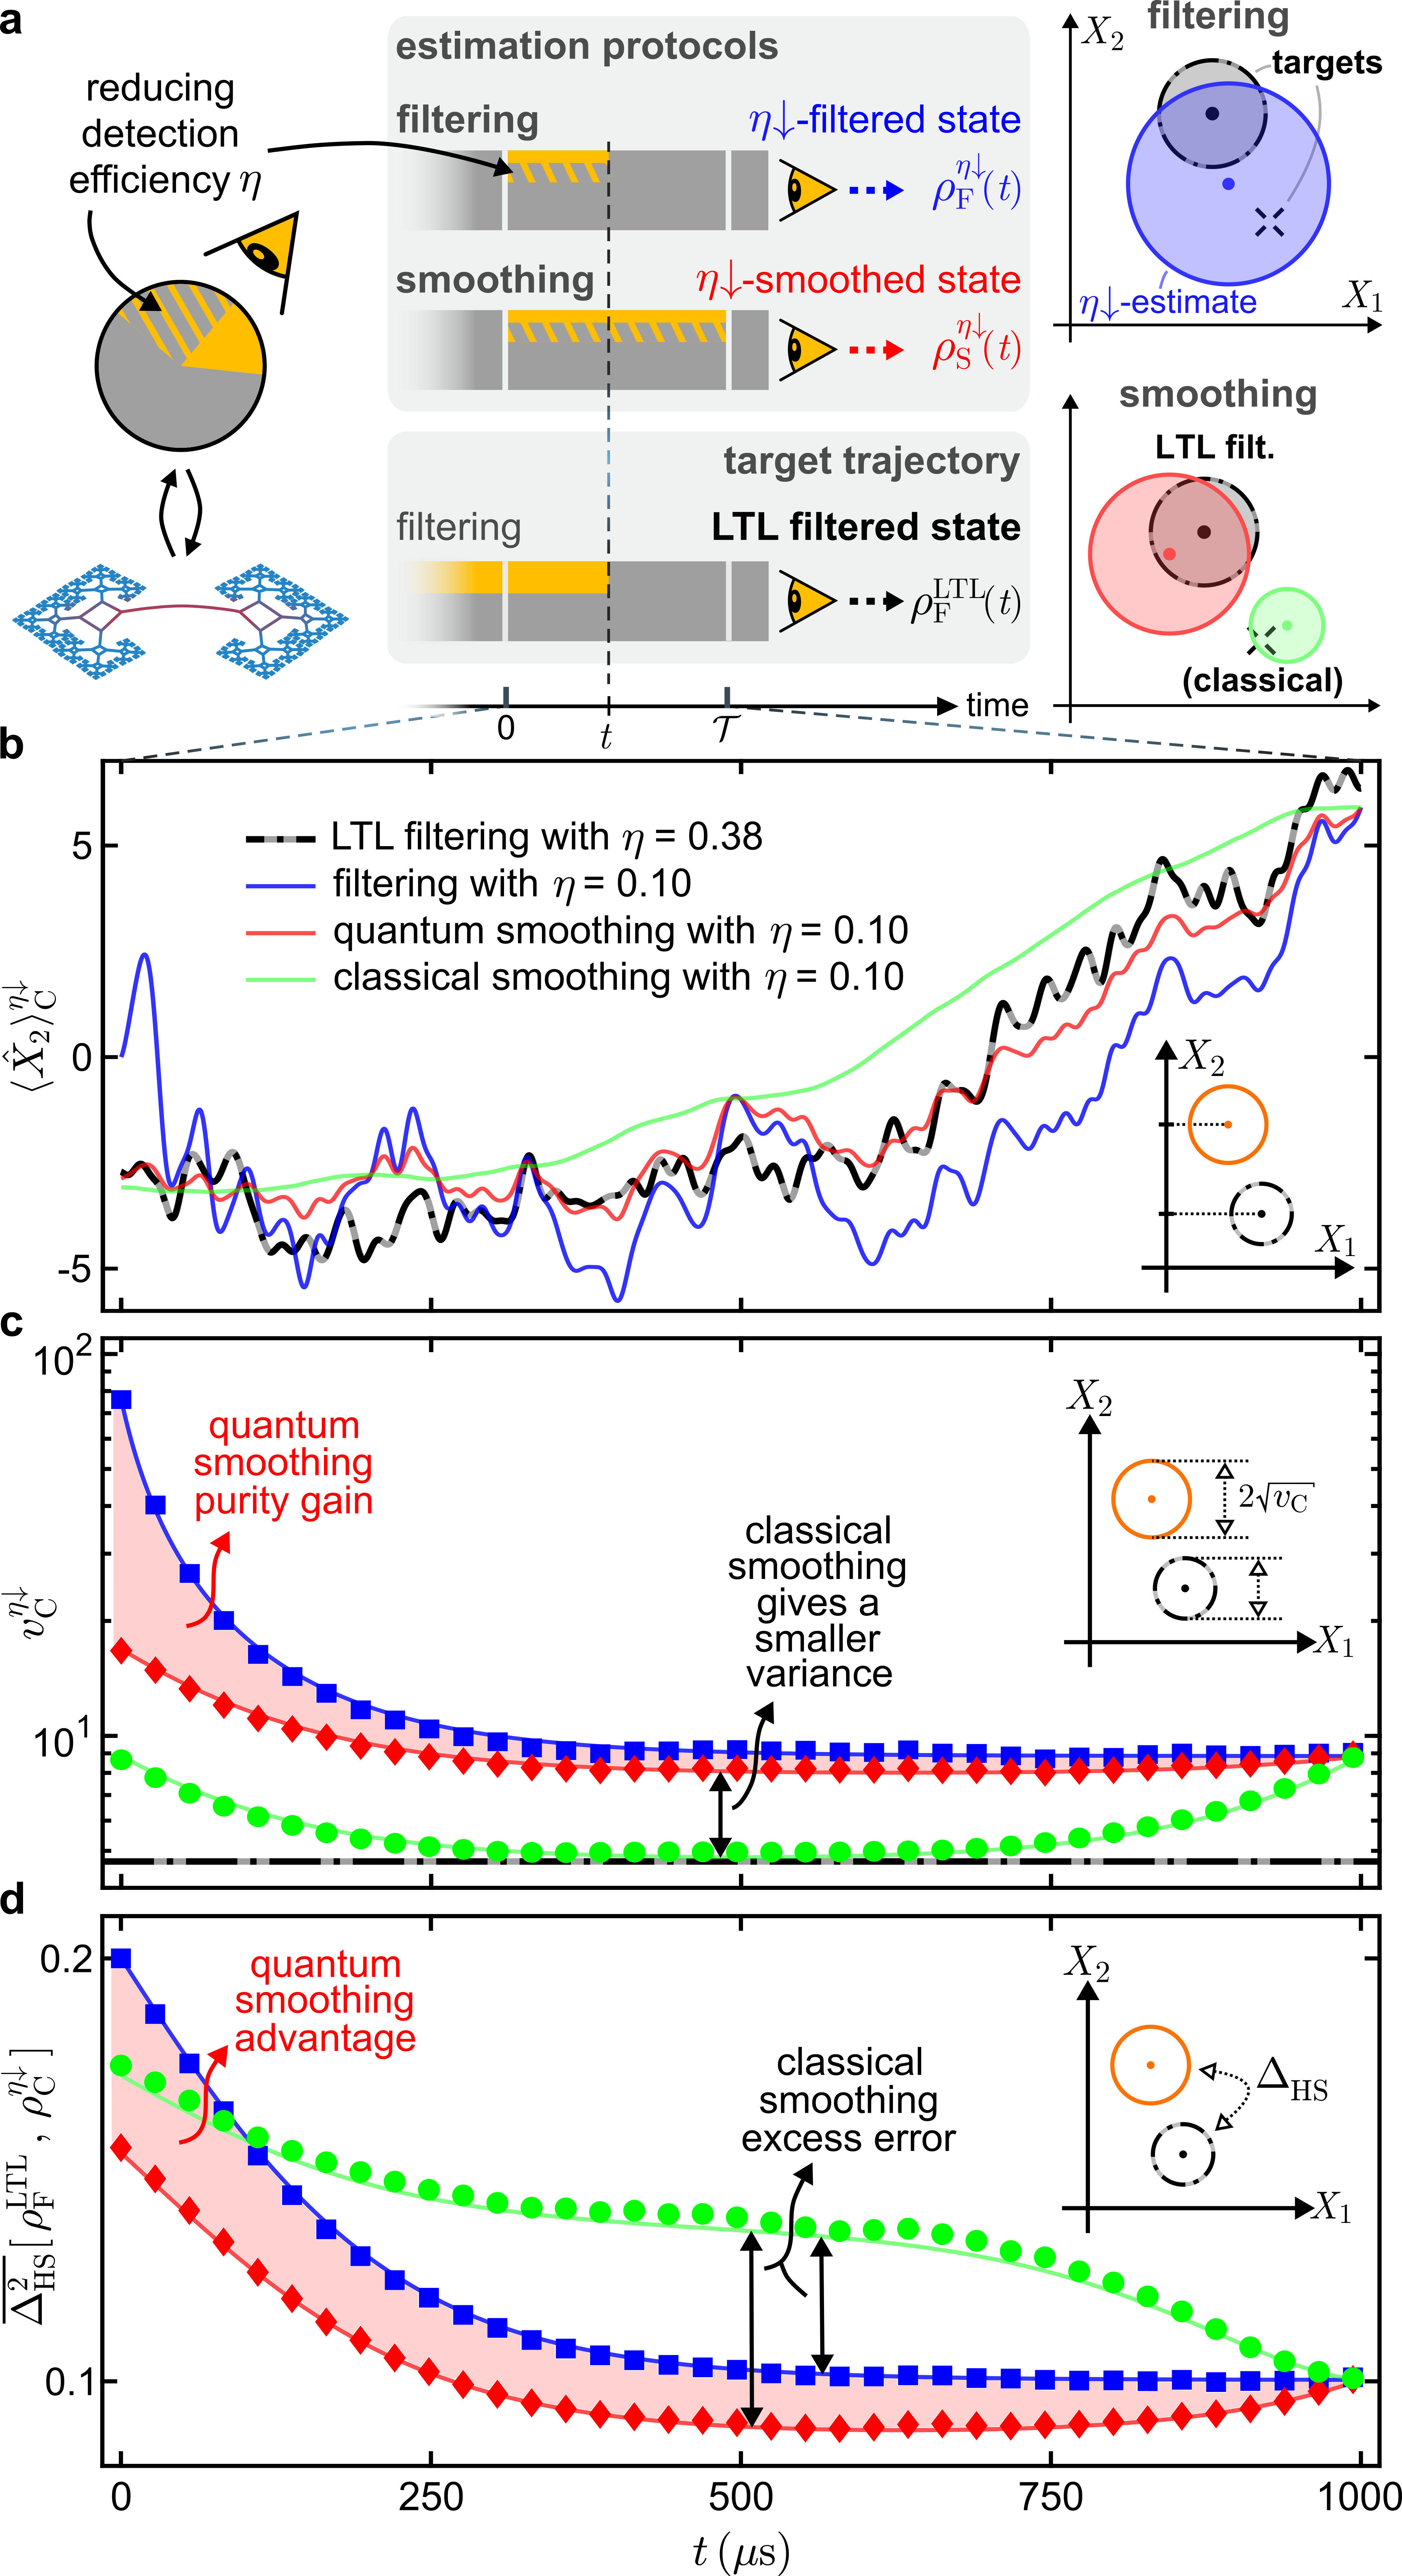
\includegraphics[width=\linewidth]{FigData3.png}
    \caption{
\textbf{Trajectories after noise injection.} \textbf{a,} Conceptual illustration. The yellow portions of each bar denote the measured bath fraction used to infer a quantum state for the resonator at record time $t$ (dashed line). The gray shading indicates an artificial reduction of the detection efficiency $\eta$, implemented by adding white noise to the photocurrent. This noisier current is used to estimate the trajectory of the primary LTL filtered state, a target effectively conditioned on a partially unobserved bath (similar to the ``true" target in FIG.~\ref{FigData1}). The filtered estimate (blue) relies on real-time data, whereas the smoothed estimate (red) incorporates the entire data record in post-processing. As shown in phase space (right), the filtered state also yields the optimal estimate of the fictitious true value (cross) of the resonator’s classical counterpart, which has its own smoothed estimator (green). 
\textbf{b-d,} Estimation analysis. The right insets show the quantity plotted, obtained from estimator (orange) and target (black) states. 
\textbf{b,} Stochastic quadrature means $\langle\hat{X}_2\rangle_\text{F}^\text{LTL}(t)$ and $\langle\hat{X}_2\rangle_\text{C}^{\eta\downarrow}(t)$, with C = F (filtering), S (smoothing) or cS (classical smoothing), shown for a sample measurement record. 
\textbf{c,} Deterministic variances of the target, estimator states, and classical smoother. The values of $v_\text{C}^{\eta\downarrow}$ agree well with $\sigma^2_\text{uncon}-\mathbb{V}\text{ar}_{\text{ens}}[\langle\hat{X}_j\rangle^{\eta\downarrow}_\text{C}(t)]$ computed over an ensemble of 12,489 records (data points, Supplementary~\ref{SecConsistency} and \ref{sec:ErrorBars_forSC}). The similarity in variance between the target and classical smoother is coincidental. \textbf{d,} Comparison of the estimator states and the classical smoother with the target. The data points represent the ensemble average of the Hilbert–Schmidt distance squared, $\Delta^2_\text{HS}[\rho_\text{F}^\text{LTL}(t),\rho^{\eta\downarrow}_\text{C}(t)]=\text{Tr}[(\rho_\text{F}^\text{LTL}(t)-\rho^{\eta\downarrow}_\text{C}(t))^2]$. Theoretical predictions are shown as lines.}
    \label{FigData3}
\end{SCfigure*}

Therefore, as a final experiment to demonstrate the performance of our true-state estimators, we add white noise to the homodyne photocurrent. This effectively creates an additional unobserved bath whose measurement outcomes are already incorporated into the resonator’s LTL filtered state $\rho_\text{F}^\text{LTL}$. The LTL trajectory thus serves as a true-state target for the noise-added data, being partly conditioned on an unobserved bath (FIG.~\ref{FigData3}\textbf{a}). This enables direct experimental validation of our true-state estimation techniques.

The noise-added photocurrent is analysed in a similar manner to previous experiments (Methods~\ref{sec:NI_analysis}). The noise-added smoothed mean values typically track the LTL filtered state more closely than the noise-added filtered values (FIG.~\ref{FigData3}\textbf{b}), and the smoothing variance is smaller than the filtering variance (FIG.~\ref{FigData3}\textbf{c}). To quantify the performance of these noise-added state trajectories in estimating their target, we calculate their squared Hilbert–Schmidt distance to the LTL filtered state, averaged over all available records. As shown in FIG.~\ref{FigData3}\textbf{d}, it is 23\% smaller for smoothing (red) than for filtering (blue) at the record start ($t=0$) and 13\% smaller in the steady state ($t \approx 500\,\mu$s). This result validates the advantage of smoothing for estimating a true state. Significantly, it demonstrates that post-processing can partially compensate for noise-induced degradation in the accuracy of quantum trajectories. Since the effect of increasing white electronic noise is quantitatively equivalent to reducing optical detection efficiency --- in our case lowering $\eta$ from 0.38 to 0.10 (Methods~\ref{sec:NI_analysis}) --- it further indicates that post-processing can mitigate any bath measurement inefficiency.

\section{Contrasting quantum and classical smoothing} \label{Sec:traj}

%\hmw{The non-differentiability thing is interesting, but if you had to cut material from the main text this is what I would cut.}
The filtering equations that apply to linear-Gaussian quantum systems are the same as those of classical dynamical systems, as the measured observables of the bath commute with the past Heisenberg-picture observables of the system~\cite{wiseman2009quantum}. However, they do not commute with the future observables, and thus quantum state smoothing cannot be regarded as a direct extension of classical smoothing~\cite{guevara2015quantum}. This leads to characteristic differences.

One key difference is that the quantum-smoothed mean values are predicted to generally exhibit stochastic character (with special exceptions identified in Ref.~\cite{laverick2021quantum}). By contrast, classical smoothing yields mean value traces that are --- as the name suggests --- smooth, with a first derivative that is continuous in time (except in the presence of correlated measurement and process noise~\cite{laverick2021quantum}). To validate these theoretical predictions, we apply the classical smoothing equations, given by Eq.~\eqref{QSSforLTLfil} with all $\mathbf{V}\fil^\text{ss}$ terms replaced by $\mathbf{0}$~\cite{fraser1969optimum}, to our measurement records. As the feedback-induced correlation is negligible, the trajectories of the classical mean values are indeed smooth, with no abrupt changes in the time derivative (green lines in FIGs.~\ref{FigData1}\textbf{b} and~\ref{FigData3}\textbf{b}). The stochastic behaviour of the quantum traces should, in principle, manifest as sharp features with an ill-defined time derivative. While the finite acquisition speed of any real experiment prevents such sharp features from being directly observed, signatures of the stochastic behavior are evident in our experiment as enhanced fluctuations of the mean values, i.e., faster changes in the time derivative of all red curves in FIGs.~\ref{FigData1}\textbf{b} and \ref{FigData3}\textbf{b}. 

To compare the fluctuations quantitatively, we compute the autocorrelation of the time derivative of the mean values, or ``quadrature velocities". The autocorrelation functions for the noise-injection experiment are shown in FIG.~\ref{FigData4}. As expected, the quadrature velocities for classical smoothing exhibit sustained correlations, with a 115-$\mu$s decorrelation time. By contrast, both quantum smoothing and filtering show rapid decorrelation, about 21 times faster than classical smoothing and consistent with the experimentally acquired noise. Thus, our experiment verifies one of the key expected differences between classical and quantum smoothing.

\begin{figure}
    \centering
    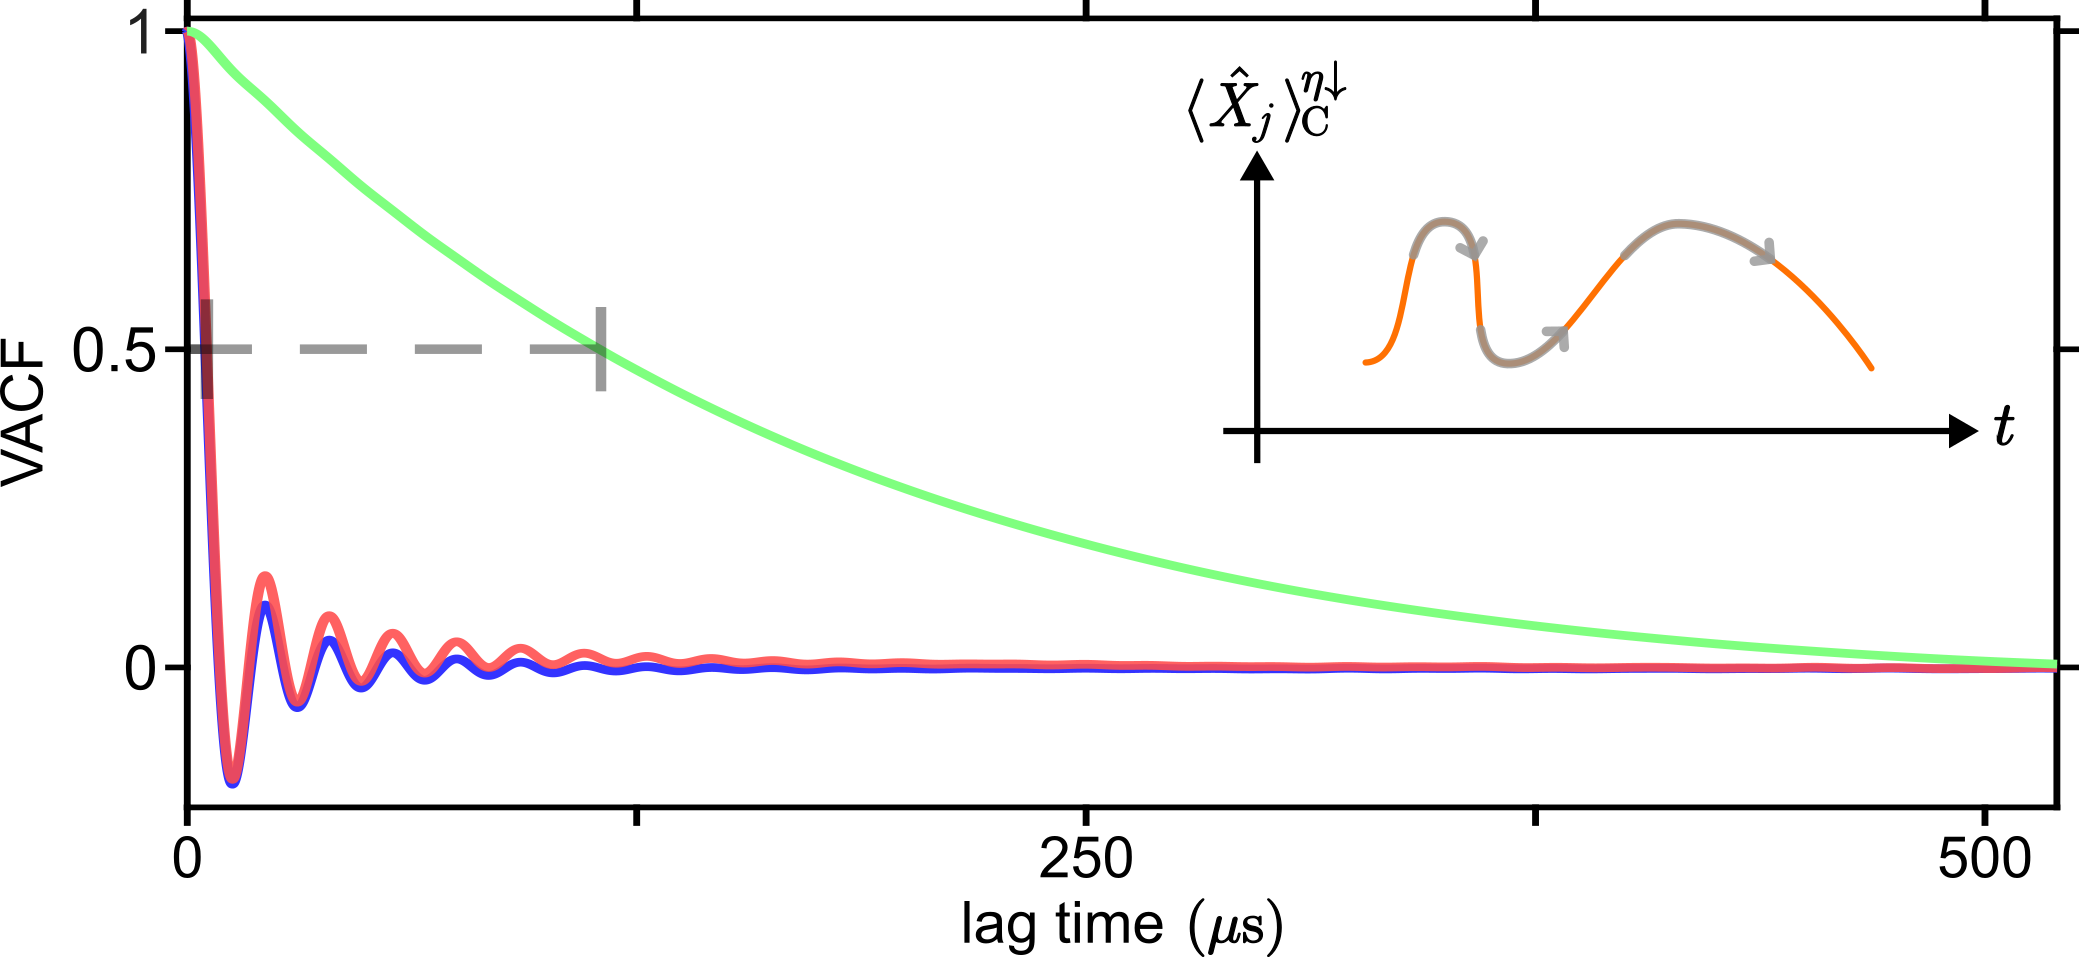
\includegraphics[width=\linewidth]{FigData4.png}
    \caption{\textbf{Fluctuations of the mean value traces.} The quadrature ``velocity" $(\dd\langle\hat{X}_j\rangle_\text{C}^{\eta\downarrow}/\dd t)$ autocorrelation function (VACF) for filtering (blue), quantum state smoothing (red) and classical smoothing (green). Its decay, indicated by the dashed line, is markedly slower for classical smoothing. The function is first averaged over $j$ and across the ensemble of measurement records in the noise-injection experiment, and then normalized to its maximum value.} 
    \label{FigData4}
\end{figure}
%\ktl{Hmm, I wonder if it is not better to plot $|{\rm VACF}|$ and take the correlation time of the envelope? Also this seems just a fraction blurrier than the other figures (not major). I also wonder if we should print the value of the length of the grey bar on the plot?}
A second key distinction is that the classical smoothing equations --- when applied to a quantum system --- can produce unphysical quantum states. In fact, the classical smoothing variance can fall below the minimum value set by the Heisenberg uncertainty principle (see Discussion and Ref.~\cite{LCW25}). Our experiments show precursors of this apparent violation of the uncertainty principle in FIGs.~\ref{FigData1}\textbf{d} and~\ref{FigData3}\textbf{c} where the classical smoothing variances (green curves) are consistently smaller than both quantum smoothing and filtering. Additionally, the classical mean values (green lines in FIGs.~\ref{FigData1}\textbf{b} and~\ref{FigData3}\textbf{b}) --- while giving the \textit{weak values} of the quadratures~\cite{tsang2009optimal,LCW25} --- are not optimal estimates of the mean values of the target states. For example, the green circles in FIG.~\ref{FigData1}\textbf{c} show the statistical deviation of the mean values when targeting the LTL filtered state, demonstrating their inferior accuracy compared to quantum state smoothing. Finally, the larger squared Hilbert-Schmidt distances for classical smoothing (green curves in FIGs.~\ref{FigData1}\textbf{d} and~\ref{FigData3}\textbf{e}) confirm that the trajectories produced by the classical equations are more distinguishable from the targets than the quantum smoothed trajectories. These experimental findings highlight the fundamental inadequacy of classical smoothing for reconstructing quantum state trajectories.

\section{Discussion}

Our demonstration that future information allows more accurate quantum state trajectories could enable a range of new applications in quantum sensing, communication and computation~\cite{Duan2025concurrent, Sayrin2011realtime,Magrini2021realtime,convy2022machine,livingston2022experimental}. For instance, in quantum sensing, it may allow improved precision. We validate this, in spirit, in the noise-injection experiment, where future information is used to mitigate noise, improving the precision with which the quadrature mean values are known.
%improving the reconstructed trajectory of the state.
In quantum error correction, it may benefit protocols that employ post-processing~\cite{convy2022machine,livingston2022experimental}. These protocols must store information, presenting resource constraints for large-scale quantum computers. Here, trading off some stored past data for future data may allow a net reduction in the stored information for post-processing with a desired level of accuracy.

Our approach is particularly relevant to protocols that exploit the transient conditional dynamics of quantum systems shortly after monitoring begins. For example, continuous weak measurements are widely used to generate non-classical states of quantum systems~\cite{muller2008entanglement,meng2020mechanical,thomas2021entanglement}. 
%{\color{blue} Evolution towards the desired state occurs transiently over time.} \skh{Honestly, honestly: I needed a lot of time to understand what you by this sentence and that adverb `transiently'. What does happen if we remove this sentence?} 
Employing future information could allow useful states to be produced earlier in the transient phase and improve the fidelity of the final states that are generated.
%\skh{`to the desired ones.'} 
Similar transient-phase physics has been shown to play an important role in studies of conditional entropy production under weak continuous measurement~\cite{rossi2020experimental}. Since quantum smoothing yields purer quantum states, access to future information would appear to modify the rate of entropy production, offering a new perspective on these studies. 

As discussed earlier, while our formalism allows improved estimation of the true state of quantum systems that are interacting with an environment, there is usually an ambiguity about the type of the true state. This raises interesting philosophical and practical questions about decoherence in quantum mechanics. In particular, different assumptions about the nature of the unobserved environment lead to different sets of possible true states, even when the observed measurement record is identical. For instance, while an environment that performed position detection would drive the resonator towards a coherent true state~\cite{bowen2015quantum}, phonon-number resolving measurements would instead drive it towards a Fock state~\cite{brawley2016nonlinear,deleglise2008reconstruction}. This highlights that, when adapted to the case of a single observer, quantum state smoothing is not necessarily a reconstruction of objective reality but rather a conditional description that depends on the physical model of the interactions between system, bath and environment.

Our work also highlights the incompatibility of classical smoothing with quantum state trajectories, in particular by showing precursors of the apparent violation of the Heisenberg uncertainty principle by classical smoothing. As derived in Supplementary~\ref{sec:SSvariances}, such a violation would require $\eta>0.25$ and $\mathcal{C}/n_\text{th} > 1/(4\eta-1)$. Our experiment satisfies the first condition ($\eta=0.38$) but not the second, the latter being limited by the maximum optical power that can be used before mode competition degrades performance~\cite{khademi2024optomechanical}.

%{\color{gray}Our work also highlights the incompatibility of classical smoothing with quantum state trajectories – that is, while they produce the weak values of the quadratures~\cite{tsang2009optimal}, they do not provide quantum state trajectories. Indeed, applying classical smoothing naively to estimate quantum states can yield predictions that break fundamental quantum constraints, for example violating the Heisenberg uncertainty principle~\cite{LCW25}. This makes quantum state smoothing essential for physically valid state estimation when future data is used. A precursor of apparent Heisenberg uncertainty violation is evident in our experiments in FIGs.~\ref{FigData1}\textbf{d} and~\ref{FigData3}\textbf{c}, where the classically smoothed variances are lower than their quantum counterparts. As derived in the Supplementary Section~\ref{sec:SSvariances}, a true violation would require an overall detection efficiency $\eta>0.25$ and measurement strength $\mathcal{C}/n_\text{th} > 1/(4\eta-1)$. Our main experiment satisfy the first condition ($\eta=0.38$) but not the second, the latter being limited by the maximum optical power that could be used before mode-competition degraded performance (Methods Section~\ref{?}).}

%By better estimating the LTL filtered state trajectory with the future measurement data, we showed how the system evolution can be described with less uncertainty in the transient phase. This is a novel tool for interpreting the results of quantum monitoring experiments. For example, Ref.~\cite{thomas2021entanglement} reports an experiment in which an atomic spin ensemble and a mechanical resonator are monitored by a single weak probe. The two systems, prepared in an unconditional separable state, are found in a conditional entangled state about 15 $\mu s$ after the observer starts to filter the measurement current. We can then ask whether the systems were actually entangled during this transient time or not. Such questions raise a discussion around the (subjective or objective) reality of the systems' trajectory. Measuring the time needed for the systems' smoothed quantum state to show conditional entanglement will offer a new perspective on this discussion, because the smoothed quantum state better represents the systems' evolution based on the same measurement record. Another example is the experimental study of the change of entropy in a monitored mechanical resonator in Ref.~\cite{rossi2020experimental}. It is shown that the rate of \textit{irreversible entropy production} is smaller in the transient phase of the filtered dynamics, compared to the unconditional dynamics, and the difference is linked to the information obtained via the continuous measurement. Given that our quantum state smoothing technique can present a purer picture of resonator's conditional dynamics, calculating the entropy production rate of the quantum smoothed trajectory might lead to a deeper understanding of this link. These examples from the literature show the potential of our quantum state smoothing techniques for exploring new physics problems.

%With the concept of the true state of a quantum system, there are subtleties involved that are better clarified by contrasting to classical systems. Similar to classical estimation, the unconditional state cannot present a proper picture of the system's time evolution. For example, the unconditional state of our resonator is a thermal state and static in the interaction frame. It does not show any evolution while we know that the resonator is being kicked by the thermal and optical noises. Unlike the classical estimation though, the ideal picture of evolution is not unique for quantum systems. Classical systems have a true value but quantum systems can have different true states. For example, the true state of a resonator like ours can be a coherent state with continuously diffusing mean values or a Fock state with a continuously jumping number or the like, based on the type of measurements performed on all the baths. Nonetheless, there is a sensible choice for the true state, the purest one that is found by complementing the actual measurement, and no matter which true state is chosen to be estimated, the experiment evaluating the estimation is unambiguous. In this paper, we chose a displaced ground state as the true state of the resonator mainly because it is a pure state that would be found by complementing our actual measurement---and also because the same state would be arguably found if we had access to the output of naturally-occurring measurements.

%For our mechanical resonator in the lab, a displaced ground state was taken to be the true state. In fact, we pictured our quantum system as a harmonic oscillator that has been heated up from its ground state, only because of the back-actions of the continuous measurements being performed on it via different baths (Methods). This picture is an extended version of the terminology `back-action heating' in optomechanics literature, referring to the heating caused by the optical bath no matter what portion of the bath (characterized by $\eta$) ends up being observed.
%The system is thus pictured as a harmonic oscillator heated up from its ground state only by the back-action of the measurements performed on it. This is a generalization of the terminology ‘back-action heating’ in optomechanics literature, referring to the heating caused by the optical bath---the mean number of resonator's phonons equals $n_\text{th}+\mathcal{C}$.

%Although the classical smoothing PDF doesn't serve the purpose of this work, its first moments play a role in linear Gaussian quantum systems like ours. These moments equal the \textit{weak values} of the system's position and momentum (or its quadratures)~\cite{tsang2009optimal}. The PDF covariance matrix does not have a general function, to our knowledge, and can violate the Heisenberg uncertainty principle~\cite{tsang2009optimal,laverick2019quantum,laverick2021quantum}. {\red [Kiarn, you have duplicated refs: [27] and [29].]}\ktl{Well, this is the only way in LGQ systems that you can tell it is an anamolous effect. In finite dimensional systems, the weak-value itself tells you that it is anomolous (existing outside the eigen-spectrum) but for CV systems, the eigen-spectrum is infinite and thus it can never be outside the spectrum. well that is not true either ... hmmm. Maybe phrasing this as an indication that it is anomolous is better.}\ktl{Well, yes that is one thing, but I was actually thinking of a different question: in a CV system, how do you tell if a weak-value is anomalous? In DV this is well defined since it is defined by being outside the eigenspectrum, but in CV the eigenspectrum is unbounded. Now, certainly one way to tell would be to show that the state that describes the statistics of the WVs is unphysical, but that is probably overkill. I was thinking that maybe the classically smoothed variance would be an indicator of this (i.e., if $V_{SWD} + (i\hbar/2) \Sigma  \ngeq 0 \implies V_{SWV} + (i\hbar/2) \Sigma  \ngeq 0$ --- at least for LGQ systems). But this is not necessary for this paper at all.} For a resonator like ours, the violation happens once $\eta>0.25$ and $\mathcal{C}/n_\text{th}>1/(4\eta-1)$ (Methods). In the experiment, we accomplish a detection efficiency larger than the violation threshold but $\mathcal{C}/n_\text{th}$ remains smaller. While pumping more photons into the cavity could make $\mathcal{C}$ large enough, we avoid a stronger pump because of the subsequent contamination of the measurement signal by a higher-order mechanical mode of the device~\cite{khademi2024optomechanical}. Nonetheless, the mere possibility of violating the uncertainty principle is yet another indicator that classical smoothing equations cannot provide a better picture of the system's forward-in-time evolution.
%Our analysis also demonstrated the differences between the quantum state smoothing techniques and the classical smoothing equations. We note that the first moment of the classical smoothing PDF equals the weak values of $\mathbf{\hat{x}}$ in linear Gaussian quantum systems~\cite{tsang2009optimal}. Furthermore, it turns out that, for our mechanical resonator, this PDF is mathematically equal to the `past probability' of intermediate projective quadrature measurements~\cite{zhang2017prediction}. Past probability is the probability distribution of finding a specific outcome for an intermediate single-shot measurement conditioned to the past and future monitoring data~\cite{gammelmark2013past}. Given that the resonator trajectory has not been disturbed by such an intermediate measurement, the past probability interpretation does not physically apply to our experiment.

%{\blu Another feature we see exhibited in the data is the difference between the smoothness (in the mathematical sense) in the trajectories of the classical and quantum smoothed means. It is known~\cite{laverick2021quantum} that the classically smoothed mean will be {\textit smooth to first order} (meaning that only the mean and its derivative are continuous and differentiable over the entire evolution) provided the measurement induces no back-action (Methods) on the system. This is exactly the case for our system, and we see that the classically smoothed mean (green line in FIGs. \ref{FigData1}\textbf{b} and \ref{FigData3}\textbf{b}) is indeed smooth to first order, lacking sudden changes in the gradient of the mean. In the quantum case, however, the constraints are stronger, requiring that the target state is an eigenstate of the measured Lindblad operator \ktl{(I don't like this phrasing will fix later)}, which is not possible for heterodyne measurements since $a^\dagger$ has no eigenstates. Hence, we expect the quantum smoothed mean to behave more stochastically, with discontinuities in the derivative of the mean. Unfortunately, the quantum smoothed mean (red line in FIGs. \ref{FigData1}\textbf{b} and \ref{FigData3}\textbf{b}) is also smooth, with no discontinuities in the derivative. This is likely due to the band-pass filtering of the measurement current during the data analysis (Methods) which has softened the sharp stochastic features of the measurement record. Similar softening of the stochastic features are observed in the filtered mean. Nevertheless, remnants of this effect can still be seen through the rapidly changing gradient of the quantum smoothed mean throughout the evolution, compared to the classically smoothed mean.}\ktl{What are your thoughts on this?} 

%Despite the common case of quantum state smoothing, classical smoothing almost always \ktl{No, not almost always. Classical smoothing will only output a smooth trajectory if there is no measurement back-action, i.e. ${\bf \Gamma} = 0$, which is the case here. As soon as there is measurement back-action then the classically smoothed mean will be stochastic. Now, for classical systems such a measurement generally exists, but for quantum systems this is not the case and there will usually be a back-action term.} outputs first-moment trajectory curves that are \textit{mathematically smooth to the first order}~\cite{laverick2021quantum}. While the experimental first-moment trajectories of our resonator PDF are mathematically smooth, as expected, it turns out the experimental quantum state smoothing ones are mathematically smooth too, contrary to the theoretical prediction. This contradiction is perfectly explained by the band-pass filtering of the measurement current during the data analysis (Methods). Nonetheless, the predicted difference in the mathematical smoothness of the smoothed trajectories is still experimentally reflected by the excess fluctuation of the quantum ones in FIGs. \ref{FigData1}\textbf{b} and \ref{FigData3}\textbf{b}.

%%Our experiment can also be viewed as the process of picturing quantum decoherence. Given the resonator's master equation, a thermal distribution of coherent states constitutes a \textit{physically realizable ensemble}~\cite{wiseman2001inequivalence}, we can argue that our quantum state smoothing technique is also better picturing the natural decoherence process of the resonator.
%The framework of this paper also clarified how filtering, as the usual conditioning process, can be viewed as an explicit estimation protocol in which a purer quantum state of the system is estimated by the past measurement data. This sheds new light on the historical terminology `quantum state estimation'. A better estimate of the quantum state is found by our quantum state smoothing techniques. These are expected to find conceptual and technological applications, as novel methods of post-processing measurement records.
%%For example, in reference~\cite{rossi2019observing}, a mechanical resonator is monitored and the future record is utilized to approximately verify the value of $v\fil^\text{ss}$ (Methods).

\section*{Acknowledgements}

\noindent
We thank A. C. Doherty, W. W. Wasserman, A. G. White, I. Marinković, G. I. Harris and J. S. Bennett for useful discussions. This research was supported primarily by the Australian Research Council Centre of Excellence for Engineered Quantum Systems (EQUS, CE170100009). It was also supported by the Air Force Office of Scientific Research under award number FA9550-20-1-039, and the Australian Research Council Centre of Excellence CE170100012 (Centre for Quantum Computation and Communication Technology). K.T.L. acknowledges the Plan France 2030 through the project NISQ2LSQ (Grant ANR-22-PETQ-0006) and the project OQuLus (Grant ANR-22-PETQ-0013).

\section*{Author contributions}
\noindent
S.K. conceived the concepts of LTL filtered state estimation and the noise-injection experiment. H.M.W., S.K. and K.T.L., with input from W.P.B., developed the ideas of natural measurements and estimation of a pure state. K.T.L., H.M.W. and S.K. carried out the novel theoretical derivations. S.K. applied the framework to the experiment. S.K. and J.J.S., with input from W.P.B., built the setup, characterised the optomechanical device and devised the experimental protocols. The device was fabricated by J.C., J.G. and S.G. Final data was collected by S.K. Data analysis was carried out by S.K., with additional input from K.T.L., W.P.B., J.J.S. and H.M.W. Figures were prepared by S.K., J.J.S. and W.P.B., with contributions from J.C., J.G. and S.G. The manuscript was written by S.K., W.P.B., J.J.S., K.T.L. and H.M.W. with feedback from all authors. W.P.B. and H.M.W. supervised the project.

\section*{Competing interests}
\noindent
The authors declare no competing interests.

\bibliographystyle{apsrev4-2}
\bibliography{sn-bibliography}

\section*{Methods}
\setcounter{section}{0}
\subfile{Methods-Theory}
\renewcommand{\figurename}{Extended Data FIG.}\setcounter{figure}{0}
\makeatletter
\renewcommand{\theHfigure}{ED.\arabic{figure}}
\makeatother
\renewcommand{\tablename}{Extended Data TABLE}\setcounter{table}{0}
\subfile{Methods-Experiment}
\subfile{Methods-Analysis}


\onecolumngrid
\newpage
\section*{Supplementary Information for\\Post-processed estimation of quantum state trajectories}
\begin{center}
  Soroush Khademi, Jesse J. Slim, Kiarn T. Laverick, Jin Chang, Jingkun Guo,\\Simon Gröblacher, Howard M. Wiseman, and Warwick P. Bowen
\end{center}
\renewcommand{\thesection}{S\arabic{section}}\setcounter{section}{0}
\renewcommand{\thesubsection}{S\arabic{section}.\arabic{subsection}}
\renewcommand{\theequation}{S\arabic{equation}}\setcounter{equation}{0}
\renewcommand{\figurename}{FIG.}
\renewcommand{\thefigure}{S\arabic{figure}}\setcounter{figure}{0}
\makeatletter
\renewcommand{\theHfigure}{S.\arabic{figure}}
\makeatother
\renewcommand{\tablename}{TABLE}
\renewcommand{\thetable}{S\arabic{table}}\setcounter{table}{0}
\subfile{Material_Supp}

\end{document}